% texcount ~/Work/jpr-ilc2015/manuscript.tex
% all under 10,000

\documentclass[pdftex,11pt]{article}
\usepackage[top=1in,bottom=1in,left=1.5in,right=1.5in]{geometry}
\usepackage{setspace}

% Link style
\usepackage[pdftex, hyperfootnotes=false, colorlinks=true, citecolor=dukeblue, linkcolor=dukeblue, urlcolor=dukeblue, breaklinks=true]{hyperref}
\hypersetup{%
    pdftitle={ILC 2015},
    pdfauthor={Andreas Beger,Michael D. Ward},
    bookmarksnumbered=true,
    citebordercolor={1 0 0},
    }
    
% change date format
\usepackage{datetime}
\newdateformat{mydate}{\THEDAY~\monthname[\THEMONTH] \THEYEAR}

% Better citation, set punctuation.
\usepackage{natbib}
\bibpunct{(}{)}{,}{a}{}{,}

\usepackage{pdftexcmds}

% Fonts setup
%\usepackage{fontspec}
%\setmainfont{Calibri}

\usepackage[T1]{fontenc}
\usepackage{fourier}		% serif font
%\renewcommand{\familydefault}{\sfdefault}
%\usepackage{helvet}
%\usepackage{mathptmx}	% Times serif w. maths

% Graphics
\usepackage{graphicx}
\usepackage[usenames,dvipsnames,svgnames,table]{xcolor}
\definecolor{dukeblue}{rgb}{0, 0, 0.61}
\graphicspath{{figures/}}			% location of graphics folder

% Other things
\usepackage{amsmath}
\usepackage{dcolumn}
\usepackage{xtab,booktabs}
\usepackage{rotating} % sideways tables
\newcolumntype{d}{D{.}{.}{-1}}
\usepackage[format=plain,justification=justified,labelfont=bf]{caption}
\usepackage{endfloat}
\usepackage{subcaption}
\usepackage{floatrow}
\floatsetup[table]{capposition=top}
\floatsetup[figure]{capposition=bottom,captionskip=0pt}

\usepackage{mdframed}

% For long table with all ILC
\usepackage{longtable}

\usepackage{multirow} % for data partitions table
\usepackage{pdflscape} % allows some pages in landscape via landscape env.
\usepackage{pbox}  % for data partition table, to allow line breaks in table cells

% For coloring table cells
\usepackage[table]{xcolor}
\definecolor{p05}{rgb}{0.75, 0.75, 0.75}
\definecolor{p10}{rgb}{0.9, 0.9, 0.9}

% Allows one-column abstract in two-column doc
\usepackage{abstract}

%   Rename bibliography section.
%\renewcommand{\bibname}{References}
\urlstyle{same}             % URLs are formatted same as text.
% Paragraph spacing
%\parskip=1em
\parindent=0.6cm

%
% Title page and TOC
%
%%%%%%%%%%%%%%%%%%%%%%%%

\title{Irregular Leadership Changes in 2015 and beyond}
\author{Michael D. Ward and Andreas Beger \\
Duke University}
\date{\mydate{\today}}
\footskip = 30pt

\begin{document}

% Switch to double column
%
\setlength{\columnsep}{20pt}
\parindent=0.68cm

\maketitle
\begin{abstract}
We forecast irregular leadership changes (ILCs)--unexpected leadership changes in contravention of a state's established laws and conventions---for the first 6 months of 2015 using predictions from an ensemble of seven split-population duration models. The data consists of monthly observations for up to 175 countries worldwide from 1991 to 2014, and include several aggregations of ICEWS event data. We used the same approach and models with out-of-sample AUC's of 0.85 for forecasts in mid-2014, and include an assessment of their accuracy here, as well as several considerations and best practices for real-world forecasting.
\end{abstract}

\footnotetext{Prepared for the University of Washington CSSS Workshop on 21 April 2015 and the PRIO Forecasting Workshop 22-24 April 2015, Oslo, Norway. An earlier version was presented at International Studies Association February 2015, New Orleans.  This research was sponsored by the Political Instability Task Force (PITF). The PITF is funded by the Central Intelligence Agency. The views expressed in this article are the authors' alone and do not represent the views of the US Government.  \emph{This is the first draft of the updated forecasts.}}

\clearpage


%
% 	Main text
%
%%%%%%%%%%%%%%%%%%%%%%%%

Over the past 12 months, there have been at least three instances of unexpected and irregular transitions between sitting leaders of states, once in Thailand, and twice in Burkina Faso. Yemen, currently in the throes of civil war, appears to have joined this list. Ukraine is still embroiled in a conflict that started when the then President was overthrown in a revolution. Although the means by which the leaders of these countries were overthrown vary, from military coups to revolutions to armed rebellion, we have for the past year and a half worked on modeling and forecasting the common outcome, which we call \textit{irregular leadership changes}, or ILC for short \citep{beger:dorff:ward:2014b}.

Modeling ILCs rather than the related processes like coups through which they can occur is an important addition to literatures that have largely been split by process for several reasons. Theoretically, processes are often not separable and co-occur. The coup in Mali in 2012 for example was driven by dissatisfaction with how the civilian government handled the Tuareg rebellion in the north \citep{nossiter:2012}, and Egypt over the past years has walked a thin line between revolution and coup amidst continuing mass protests. Trying to explain coups without considering the potential impact of mass protests and armed rebellions would thus only be a partial solution for important cases, and similarly for revolutions and rebellions. 

From a theoretical view this flows from research into the duration of political authorities, regimes, and polities.  The first in this line of research was the efforts of
Harry Eckstein and Ted Robert Gurr to specify a model of the theoretical dimensions of authority patterns \citep{eckstein:1973,eckstein:gurr:1975}.  The basic idea was to characterize situations with authority relations in terms of the underlying dimensions as a way of getting at the duration of different constellations of dimensions.  The first empirical component of this was Ted Robert Gurr's article entitled ``Persistence and Change in Political Systems, 1800-1971'' which developed the idea of calculating the half-lives of different sorts of political polities, regimes, and authorities \citep{gurr:1974}. This effort is in that theoretical tradition.

From a practical standpoint, the common outcome, ILCs, also is in itself important to model and forecast. To the extent that leaders of foreign states matter for foreign policy, we should care whether one is facing a risk of irregular and thus unexpected removal. From this perspective it is not as important how a leader is removed, but that he or she is removed. Furthermore, ILCs are often not only a result of violent and damaging processes, but the instability they cause can spark significant levels of violence and civil war \citep[256]{powell:thyne:2011} and has negative economic effects \citep{alesina:etal:1996, ulfelder:2013}.

The mid-2014 forecasts from \citet{beger:dorff:ward:2014a} are shown in Table \ref{tab:forecast}. The data are based on the \textit{monthly} level in order to be able to provide sub-annual forecasts, and aggregated to 6-month periods. The forecasts we presented were for the 6-month window from April to September 2014. One ILC occurred during this time: in May a caretaker government created after the previous prime minister Yingluck Shinawatra was removed by the Constitutional Court was overthrown by the Thai military. There were four other ILCs in 2014, two in the first quarter of the year before our forecast window (CAR an Ukraine), and two in the last quarter (both in Burkina Faso). Thailand was ranked 5th in the forecast we presented, and with hindsight we could have thus made forecasts with recall of 1 and precision of 0.2 by only presenting the top 5 predictions. At face value however, if we take the top 10 table we presented as our forecast, we achieved recall of 1 and precision of 0.1. 

\begin{table}
\caption{Top 10 forecasts for ILC between April and September 2014 (6 months) using March 2014 data} 
\label{tab:forecast}
\centering
\begin{tabular}{lr}
  \midrule
Country & Probability \\ 
  \midrule
Ukraine & 0.28 \\ 
  Bosnia and Herzegovina & 0.19 \\ 
  Yemen & 0.10 \\ 
  Egypt & 0.07 \\ 
  Thailand & 0.06 \\ 
  Guinea & 0.05 \\ 
  India & 0.04 \\ 
  Turkey & 0.04 \\ 
  Libya & 0.03 \\ 
  Central African Republic & 0.03 \\
   \midrule
\end{tabular}
\end{table}

The goal of this paper is to present updated forecasts for ILCs in 2015, and to further improve and explore the forecasting process on which they are based. Incorporating lessons from previous modeling, we will along the way touch on several questions:
\begin{enumerate}
\item How can the accuracy of forecasts be assessed in a meaningful way?
\item How should forecasts be presented?
\item What considerations are important for modeling when the ultimate goal is ensemble forecast?
\end{enumerate}

Properly, a social scientist might argue, we should proceed from theory, concepts and arguments about causal processes to data and measurement. The goal of our modeling and scope of the outcome we aim to forecast are in our opinion sufficiently unusual that we will proceed in a somewhat lopsided manner instead, first introducing our outcome and data, before discussing what theoretical framework there is or is not for predicting ILCs. Discussing the various literatures that might be relevant for ILCs without a proper appreciation of the difficulties that forecasting a broad but still rare outcome at monthly steps and in near real time entails has in our experience invariable led to the question and criticism of why we do not draw more heavily on existing, published models. The answer, to give a preview, in short is that we would love to, but cannot, without sacrificing either forecast accuracy or the ability to provide real, \textit{ex ante} forecasts, or both. 

\section{Background}

\subsection{What are ILCs?}

Irregular leadership changes are transitions between political leaders that occur outside the established rules and conventions of a state. Unlike coups or revolutions, ILC is focused on political leaders, and they can occur when a leader loses office irregularly, when a successor gain office irregularly, or, often, when both occur in succession, e.g. in a military coup in which a sitting leader is replaced by a military ruler. The concept is directly based on the classification of leader entry and exit from power in the Archigos project, which codes global state leaders and various details of their tenure in power \citep{goemans:etal:2009}.

The standard against which an entry or exit from office is judged to be regular is specific to a given country at a given time, and established by whatever written, legal, or informal but commonly accepted rules and conventional exist at that time. The focus is thus not on the rules of succession themselves, which are quite variable, for example from a hereditary monarchy like Saudi Arabia, to a established democracy like Switzerland, but rather on whether existing expectations are followed. A father-son transition might be regular in Saudi Arabia, but not in Denmark, at least without intervening fair elections and coalition formation. 

The underlying and to some degree implicit criterion is the extent to which a transition is predictable, or at least predictably unpredictable. If transitions follow some norm, however informal that norm might be, the possible range of outcomes will be circumscribed. In highly formal systems, like the US, it might be possible to anticipate Presidential successors weeks or month ahead of time. But even in bureaucratic dictatorships with opaque procedures in narrow bodies like a central party committee, one often can identify a set of likely successors some time in advance. Irregular changes on the other hand are by definition outside the system and not predictable based on the rules governing transition. This relationship between irregular changes and predictability is in large part a reason for why being able to anticipate deviations, irregular leadership changes, are useful to forecast.  

We code ILCs based on the Archigos coding of leader irregular entry and exit. Archigos codes all effective state leaders over the period from 1875 to 2014, for all states in the \citet{gleditsch:ward:1999} list of states. The leader data also include a few other characteristics of leaders, including gender and birth dates. 

The map in Figure \ref{fig:ilc} shows the spatial distribution of ILCs from 1991, when our data start, to 2014, and Figure \ref{ilc-timeline} show the number of ILCs by year. ILCs apparel to cluster in West Africa and Central Asia, and occurred more frequently in the early 1990's, before leveling off at the current level of 3-4 per year. 

\begin{figure}
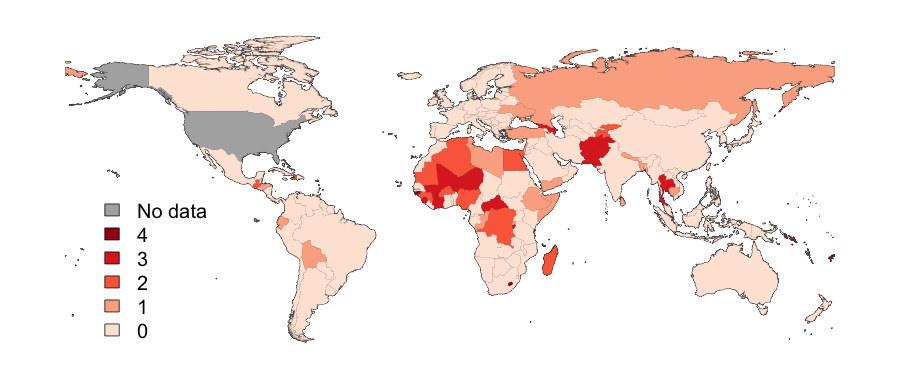
\includegraphics[width=3.2in]{ilc-map.png}
\caption{ILCs, 1991 to 2014}
\label{fig:ilc}
\end{figure}

\begin{figure}
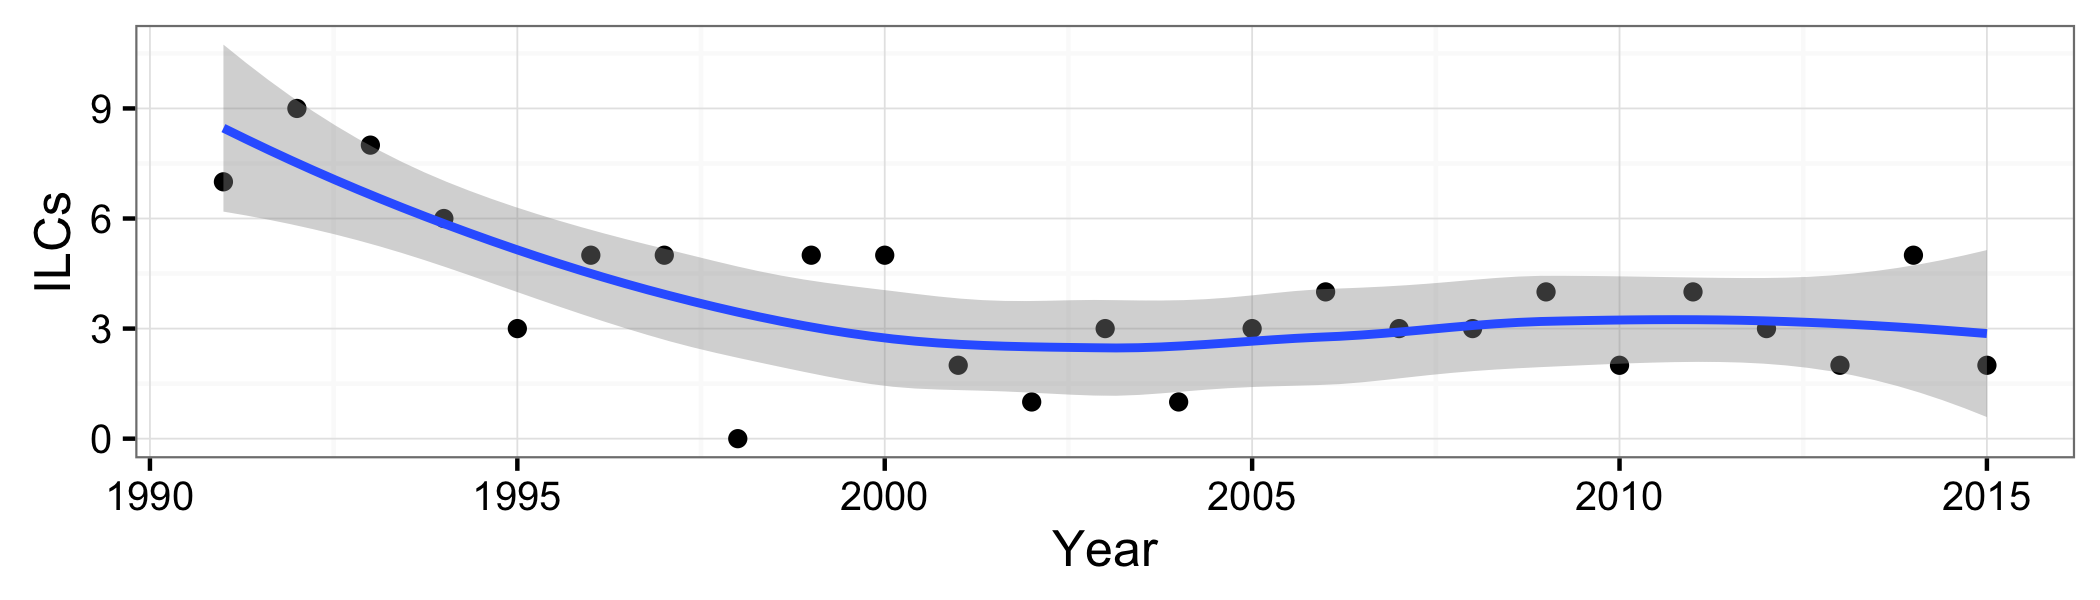
\includegraphics[width=3.2in]{ilc-by-year.png}
\caption{ILCs by year, 1991 to 2014}
\label{ilc-timeline}
\end{figure}

The concept of ILC overlaps with several subjects that have more frequently been studies in political science, including coups and rebellions. Indeed, a majority of ILCs correspond to either successful coups, where the military or other parts of government overthrew a leader, successful revolutions in which mass protests ousted a leader, or successful rebellions, where groups outside the state overthrew a leader using armed force. All three of these subjects have received considerable attention, and to some extent--limited by modeling challenges we discuss below--are relevant for predicting ILCs. 

We view the relationship between ILCs and coups, revolutions, and rebellions as one differentiated by a focus on outcome versus process. ILCs essentially are successful coups, revolutions, and rebellions, but we are less concerned with the way in which an ILC was brought about than the fact that it did occur, for the reasons outlined in the introduction.

\subsection{Data and source}

The data are based on \textit{monthly} observations of roughly 175 countries identified by the \citet{gleditsch:ward:1999} list of states from 1991 through 2014. The unit of observation is the country-month. The last observed data are in December 2014. 

The dependent variable is a binary indicator of whether an ILC occurred in a given country-month, coded based on whether Archigos codes an irregular exit or entry for the leader ruling a state.

For covariate data we draw on four main sources, the World Bank World Development Indicators \citep{wdi:2012}, Polity \citep{marshall:jaggers:2002}, Ethnic Power Relations \citep{wimmer:etal:2009}, and various indicators constructed from the ICEWS event data \citep{obrien:2010, ward:etal:2012, icews:2015:data,icews:2015:aggregations}. The resulting covariates roughly fall into three categories: structural variables, often measured annually, which are relatively stable over time and mainly vary between countries, monthly counts of various aggregations of ICEWS events, which vary widely both across time and countries, and lastly spatial lags of several ICEWS event aggregations, which have little spatial variation but vary significantly over time. 

Several countries which broke up in the early 1990's, e.g. Yugoslavia and the USSR, are missing data for the short amount of time they were in our observation window, as both of our major sources, WDI and ICEWS, have retroactive series for the successor states rather than the larger states from which they broke. For example, WDI has continuous data for Serbia into the early 90's which seem to exclude Montenegro and Kosovo, even though these were part of the larger state of Yugoslavia, later Serbia and Montenegro, and ultimately Serbia, until 2006 and 2008 respectively, and no data for Yugoslavia itself. Instead of attempting to re-aggregate such cases from individual series, we dropped the few affected country-months. 

\subsection{Methods and models}

ILCs are generally rare events, with fewer than a hundred over the past 25 years, and the data are even more sparse at the monthly level than they would be with annual data. Rare events and spares data are not unusual at all in conflict research, but the process of predictive modeling exposes several challenges this introduces. 

Furthermore, as we discussed, ILCs are outcomes that empirically are driven by many distinct processes, roughly including at least the three categories of coups, revolutions, and armed rebellions. If the processes or factors that might drive ILCs were common across the mechanisms that can lead to ILC, then it might be worthwhile to pursue a general model. \citet{cunningham:lemke:2013} provide an analogous example illustrating this thought process by arguing that civil wars and interstate wars should be studied jointly because the key causal drivers are similar across both outcome, e.g. information asymmetries. 

This is unlikely to be the case with ILCs.
%ADD 
Key factors like counterbalancing or spending priorities can have opposing effects on the chances that one of the mechanisms driving ILCs will occur. Spend a little bit more on your military and maybe the people will start protesting; create multiple, competing security organizations and maybe the chances of a military coup will decrease, but your military will be less effective in fighting an internal rebellion. These kind of dynamics require distinct models for distinct mechanisms, to allow the associated indicators to have variable effects, and a general model of ILCs thus seems unlikely. 

A brute force solution to the problem posed by the multi-causal nature of ILCs might lie with more esoteric, from a social science perspective, models and algorithms from machine learning. Methods like neural nets, SVM, and decision trees/random forests can incorporate nonlinear relationships and have been created specifically for the task of prediction. A major drawback of such methods however is that they typically are ``black box'', meaning that the mapping from inputs to outputs is complex and usually cannot be easily interpreted. This conflicts with the premium in forecasting for policymakers and other public consumers for approaches that allow statements about the underlying factors or models that drive a forecast.

We instead rely on an ensemble of several distinct models to produce our forecasts, and specifically use Ensemble Bayesian Model Averaging to transform and weight component forecasts from several thematic models \citep{Raftery:2005, montgomery:etal:2012}.

The EBMA ensemble forecast for forecasts $f_k^\prime$ from $k$ input models is a weighted average of transformed raw input probabilities using estimated weights $W$ that maximize fit over a sample of calibration data. The raw forecast probabilities first undergo an adjustment for bias reduction, $h()$, which in effect transforms the probabilities to the logit scale and pulls them closer to 0 in order to reduce the effect of extreme predictions:\footnote{The notation is largely consistent with \citep{montgomery:etal:2012} save for the use of terms to denote the transformation equations.}
\begin{eqnarray}
f_k &=& h(f_k^\prime) \\
      &=& [ ( 1 + \textrm{logit}(|f^\prime_k|))^{1/b} - 1 ] \times [ - I(f^\prime_k < 1/2) ]
\end{eqnarray}
where $b$ denotes the extent of compression, usually recommended to be set at 3 or 4, and where $I()$ is an indicator function. The logit-scale forecasts then undergo an affine transformation based on parameters from a logistic regression on observed outcomes in the calibration sample before being combined into the final weighted average:
\begin{eqnarray}
g_k(y|f_k) &=& \textrm{logit}^{-1} ( a_{k0} + a_{k1} \times f_k ) \\
p &=& \sum_{k=1}^K w_k g_k(y|f_k)
\end{eqnarray}

Given the sparse nature of the data and the insight that many countries in our data will for practical reasons not experience ILCs in the time frame we are using, e.g. Canada, we use split-population duration regressions as the workhorse of our thematic models \citep[for an application in political science, see][]{svolik:2008}. 

Split-population duration regression is a mixture of two equations, one that reflects a traditional duration model with time-varying covariates and accelerated failure time form, and a second logistic equation that simultaneously estimates the risk that a case will be at risk of failure at all. The likelihood is given as a product of the immunity $\pi$ and the risk, where $\delta_i$ indicates whether a spell ended in failure: 
\begin{eqnarray*}
\mathcal{L}\{\theta|(t_{1}, \dots, t_{n})\} &=& \prod_{i=1}^{N} \left\{(1-\pi) f(t_i)\right\}^{\delta_i} \times \\
&&   \left\{\pi + (1-\pi)S(t_i)\right\}^{1-\delta_i}
\end{eqnarray*}
Practically, the data are grouped into spells that consist of observations for a particular country over time until either ILC occurs, when a new spell starts, or until the right-censoring time. Risk is back-coded for all spells that had an observed ILC, and thus the risk variable is much more extensive than the number of observed ILC country-months itself. This allows the logistic equation to separate country-months that are likely to be in the risk or immune set. The duration equation can accommodate a Weibull or log-logistic form for the hazard function, but the Weibull shape appears to fit better in our thematic models. 

\subsection{Theme models}

Given the extensive literatures on coups, rebellions, etc., one would think that there is a fertile ground for thematic models firmly grounded in previous arguments. In practice there are two serious obstacles that have deterred us from attempting to do so, and which led us instead to largely seek our own set of thematic models. 

The first is induced by the move to monthly data, and keeping in mind that most extant models were developed and tested with yearly time-frames in mind, comes down to the simple and probably obvious point that to predict variation at the monthly level, one needs inputs that very sub-annualy \citep{beger:dorff:etal:nd}. Direct adaptions of most existing models in the literature cannot possibly be used to predict at the monthly level because these models tend to rely on structural indicators that vary little over time and in any case are often only available with annual resolution. 

The second challenge that further complicates and adaption of exiting models is that they often depend on possibly artisanal variables that are used to evaluate arguments and their hypotheses, and which often are either not available without missing data problems, or are not regularly updated and only available through a time period several years back. 

This is not to say that there are no models which use frequently updated covariates available through recent years and which could easily be augmented with event-data based indicators to help their sub-annual variance. But at this point matters become a problem of resource allocation. There is no reason to expect that models designed for causal inference will fit the data well, let alone be able to predict well out of sample \citep{ward:greenhill:bakke:2010}, and thus little guide for where to invest limited time and effort. 

As a first step, which we are still hoping to improve over time, we resorted to developing our own thematic models, partly where we could on adaptions on existing models like the political instability model in \citet{goldstone:bates:etal:2010}, or inspired by general concepts in relevant literatures like conflict contagion \citep[e.g.][]{buhaug:gleditsch:2008}, or, lastly, based on groupings of indicators like finance. 

The models reflect a tension between causal modeling versus early warning indicators that readers used to causal modeling might be uncomfortable with. Using the common example, if the goal is to predict and data are limited, then it might be alright to predict murder rates with ice cream sales, even if the relationship is spurious and driven by underlying weather patterns. Similarly, several of the thematic models include variables that might capture spurious correlations, like internet broadband subscribers per 1,000 from WDI, or to some extent tautological, like protests in the preceding month to predict the risk of mass protests that overthrow a government. 

These comments aside, the thematic models for this set of forecasts are based on updated versions of the 2014 models. One general change was necessary due to the inclusion of data for the 1990's, for which coverage in the ICEWS event data is dramatically reduced, as Figure~\ref{icews-monthly} shows. To accommodate the change in the underlying volume of events we included the total events by month for each model and equation that uses event data indicators. 

\begin{figure}
\includegraphics[width=3.2in]{icews-monthly.png}
\caption{ICEWS events by month}
\label{icews-monthly}
\end{figure}

The models otherwise are mostly unchanged, with the exception of two theme models that we will discuss with a bit more detail. Estimates for all seven models are given in the appendix, and theses also show the covariates included. For details on the model rationales, see \citet{beger:dorff:ward:2014a}.

\subsubsection{Global Instability} 

\citet{goldstone:bates:etal:2010} describe results for a predictive model of political instability, also working on behalf of the PITF. The outcome, political instability, like ILCs is an aggregate of several phenomena that have largely been studies separately: civil war, adverse regime changes, mass killings, and state collapse. The so-called Global Instability model \citep{goldstone:bates:etal:2010} use to predict instability is based on four variables, regime type, infant mortality, armed conflict in four or more bordering states, and state-led discrimination. 

We have updated the global instability model, which was very loosely based on the original effort, to more closely match the variables in the Goldstone model. The first set of variables are dummy indicators for specific types of regimes, derived from the Polity scheme: partial autocracy, partial democracy with factionalism, partial democracy without factionalism, and full democracy. These are coded based on the executive recruitment and competitiveness of political participation variables according to a table shown in Figure 1 in the Goldstone article. The other three variables in the original model are infant mortality, logged and normalized to global average by year, indicator for major conflict in four or more neighboring states, and state led discrimination using Minorities at Risk. We use the fraction of excluded population from EPR for state-led discrimination, and for the neighborhood risk indicator use two spatial weights of ethno-religious violence and rebellion in the nearest four neighboring countries.  

\subsubsection{Financial}

The original finance model included several indicators from the PITF that were not available for the 1990's. We have changed the model to instead capture oil prices (using US EIA figures), global average food prices (FAO), and local hyperinflation (via WDI) to capture financial pressures that might lead to various forms of social instability. 

\section{Forecasts for 2015}

The initial forecasts for 2015 cover the first 6 month of the year. They are based on thematic model predictions estimated using data from 1991 to 2009, and aggregated into an ensemble using an EBMA model calibrated with predictions from 2010 to April 2012, as summarized in Table \ref{timeline}. To reduce the problem of left-censoring for the duration-related variables needed to estimate the split-pop. duration regressions we use Archigos records of leadership changes back to 1955. The ensemble and component forecasts are tested against data from 2012 to 2014, before finally producing the live forecasts. 

\begin{table*}[ht]
\caption{Data partitions}
\label{timeline}
\centering
\begin{tabular}{lllp{5in}}
  \toprule
  Start & End & $t$ & Use \\
  \midrule
  1955-01 & -- & 720 & Archigos only, used to code duration and risk variables to reduce left-censoring. \\
  1991-01 & 2009-12 & 226 & Training data; estimate thematic models. \\
  2010-01 & 2012-04 & 28 & Calibration; fit EBMA ensemble using predictions from thematic models. \\
  2012-05 & 2014-12 & 32 & Test; rolling 6-month test forecasts. \\
  2015-01 & 2015-06 & 6 & Forecast period. \\
   \bottomrule
\end{tabular}
\end{table*}

\subsection{EBMA and input model results}

Table \ref{tab-ebma} summarizes the ensemble results. The first three columns list the parameters that are used to transform the component predictions into the ensemble forecast. These parameters are used to transform the component predictions, the densities of which are shown in the 7 rightmost column of Figure \ref{violin}, into the ensemble predictions, shown in the left column of the Figure. Of main interest here are the model weights, which generally give an indication of the role a thematic model plays in the ensemble. The weights are roughly related to how well a component prediction performs in the calibration period, but also how unique a model's predictions are in respect to the other models. We will return to this point later. The weight values are fairly even across models, meaning that all play at least some role in the final forecast. 

% latex table generated in R 3.1.2 by xtable 1.7-4 package
% Wed Apr  8 19:33:24 2015
\begin{table*}[ht]
\caption{Ensemble and individual models of ILCs}
\label{tab-ebma}
\centering
\begin{tabular}{llrrrrrrrr}
  \toprule
Model & \multicolumn{3}{c}{EBMA Params.} & \multicolumn{3}{c}{Calibration} & \multicolumn{3}{c}{Test forecasts} \\
  & W & a$_0$ & a$_1$ & Brier & ROC & PR & Brier & ROC & PR \\ 
  \midrule
Ensemble &  &  &  & 0.00212 & 0.880 & 0.079 & 0.0078 & 0.875 & 0.111 \\ 
  Leaders & 0.24 & 3.41 & 9.85 & 0.00216 & 0.831 & 0.013 & 0.0075 & 0.799 & 0.098 \\ 
  Public Disc. & 0.11 & 1.60 & 8.01 & 0.00218 & 0.836 & 0.022 & 0.0076 & 0.796 & 0.102 \\ 
  Global Instab. & 0.1 & -0.82 & 5.12 & 0.00217 & 0.745 & 0.013 & 0.0078 & 0.799 & 0.037 \\ 
  Protest & 0.17 & -9.30 & -2.93 & 0.00220 & 0.686 & 0.005 & 0.0079 & 0.698 & 0.051 \\ 
  Contagion & 0.15 & 0.57 & 6.30 & 0.00217 & 0.784 & 0.016 & 0.0077 & 0.873 & 0.056 \\ 
  Int. Conflict & 0.08 & -4.77 & 1.26 & 0.00217 & 0.690 & 0.008 & 0.0078 & 0.816 & 0.053 \\ 
  Financial & 0.16 & 1.09 & 6.75 & 0.00217 & 0.788 & 0.013 & 0.0077 & 0.869 & 0.056 \\    
  \bottomrule
\multicolumn{10}{p{5in}}{Note: The ensemble prediction is calculated as $p = W \times \textrm{logit}^{-1}(a_0 + a_1 f_k^\prime$)}
\end{tabular}
\end{table*}

\begin{figure}
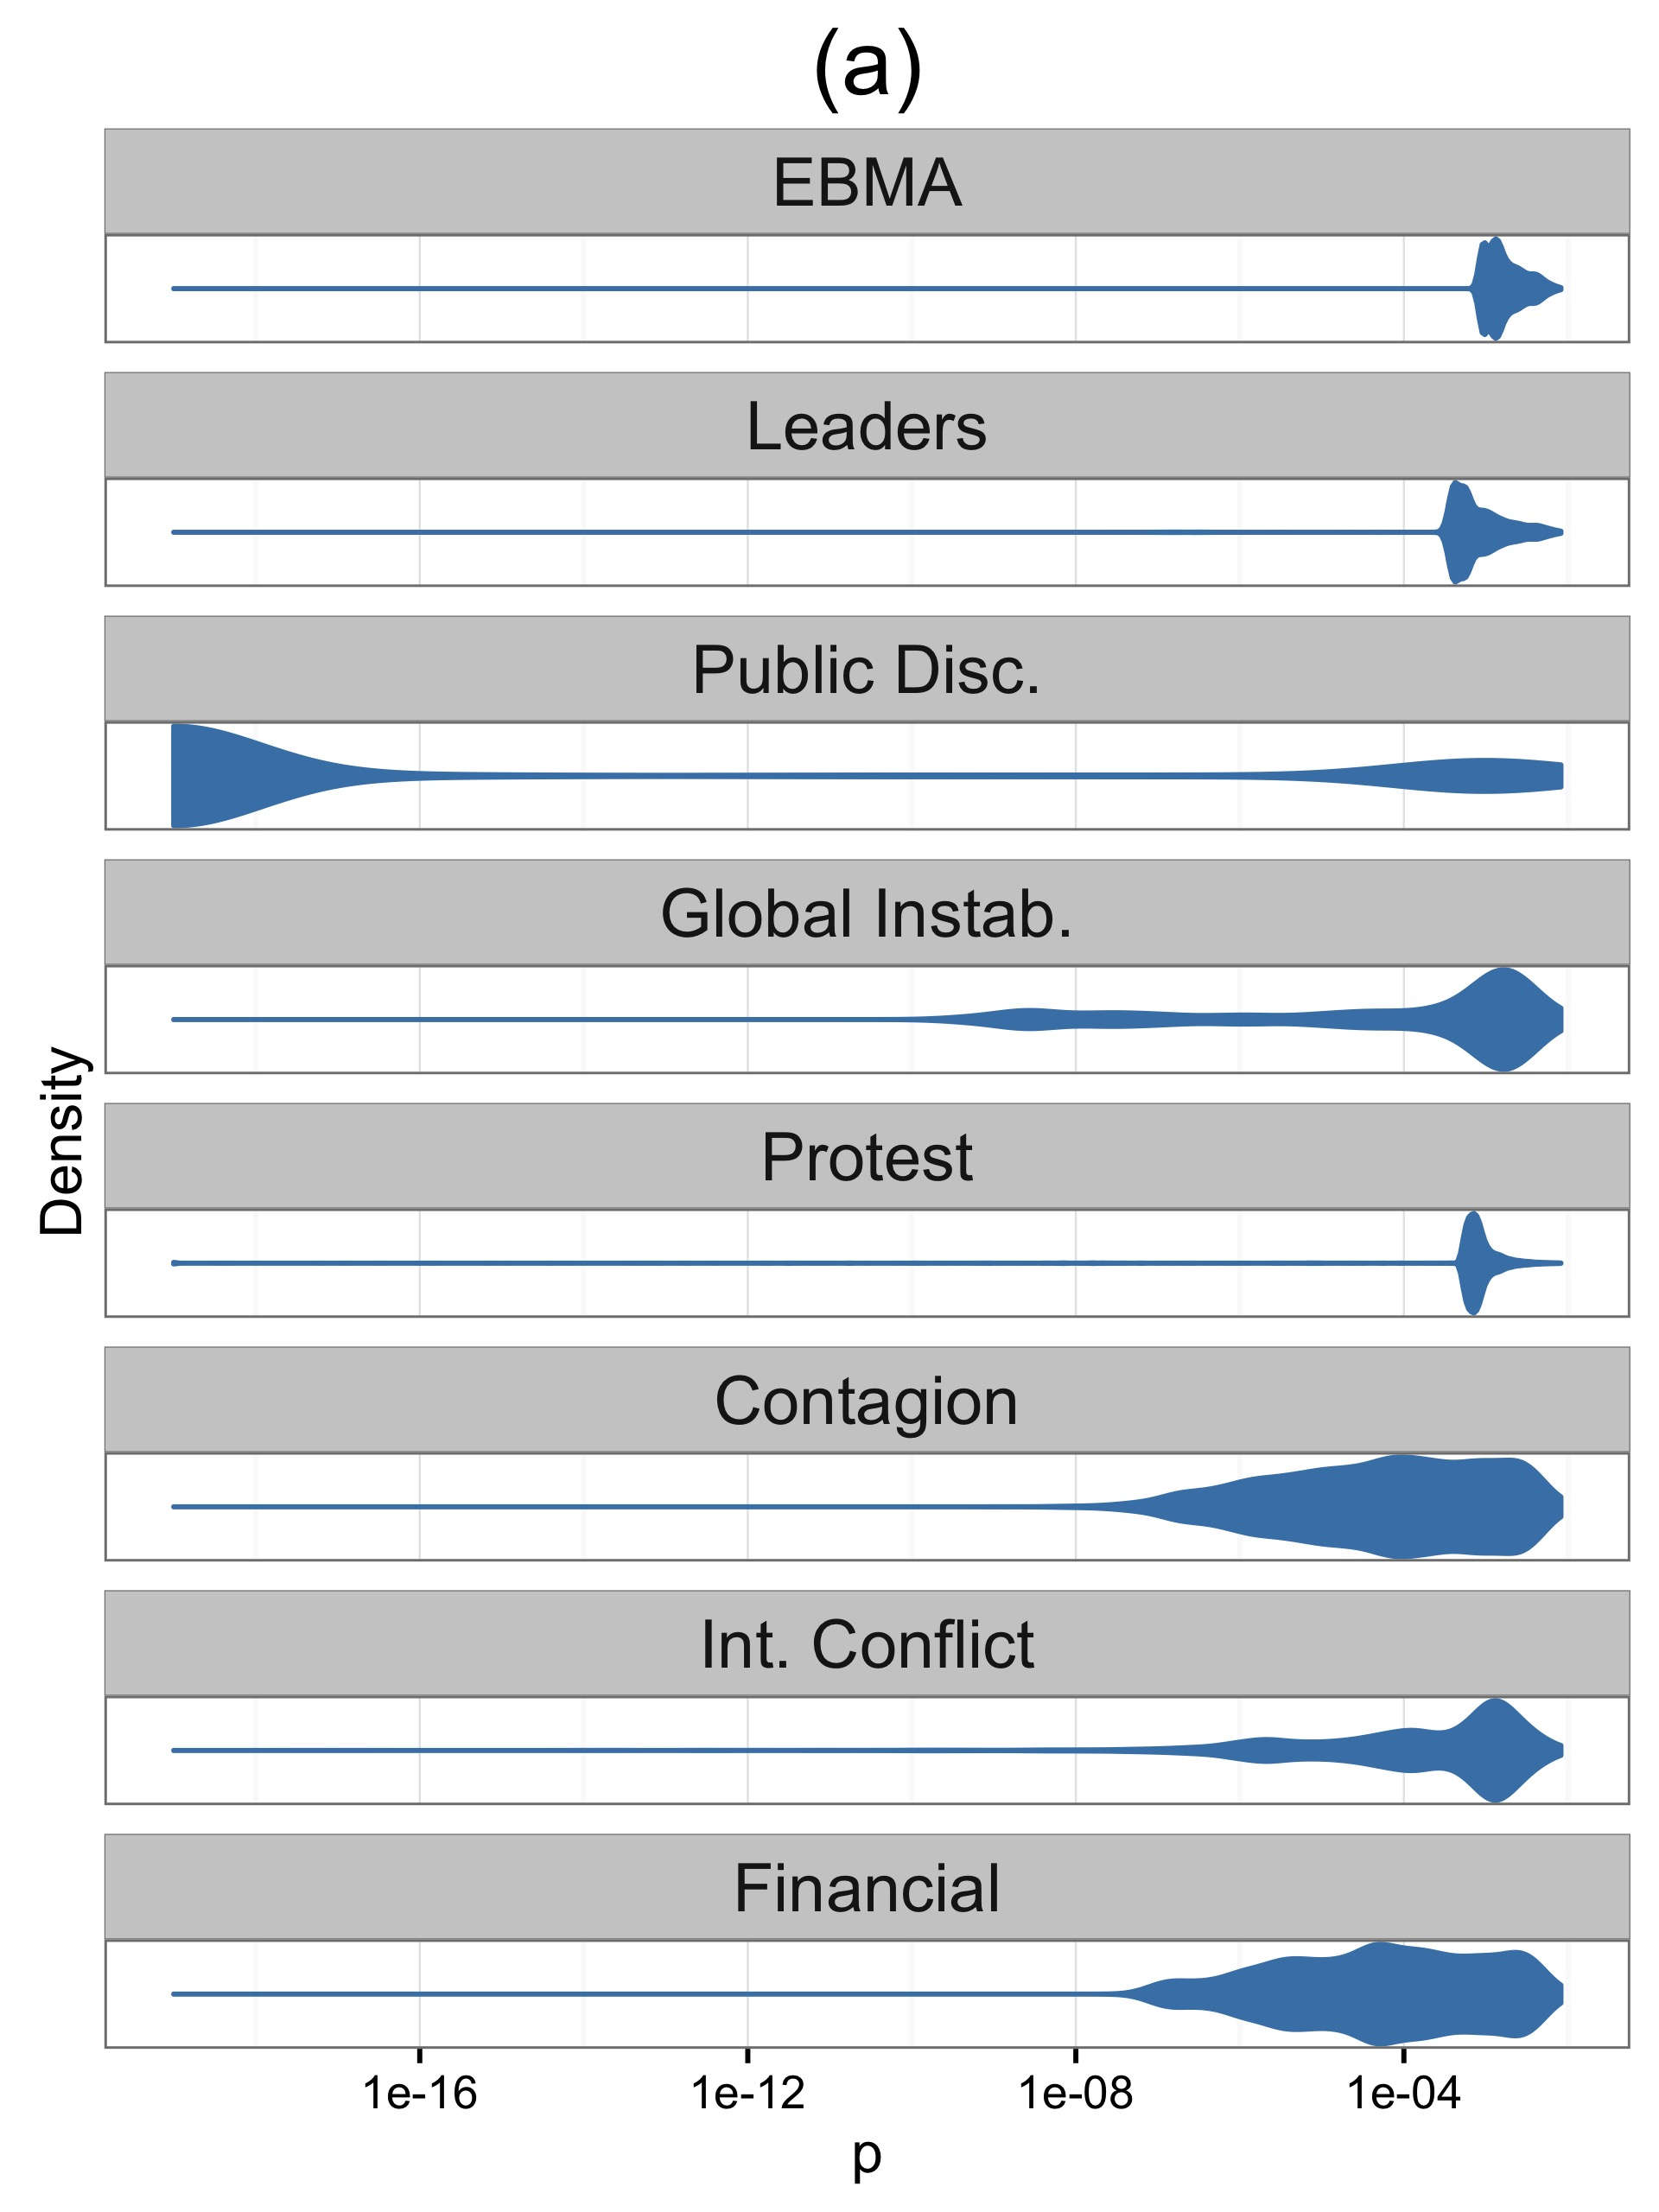
\includegraphics[width=3.2in]{p-violin}
\caption{Densities of EBMA and component model predictions}
\label{violin}
\end{figure}

To evaluate fit we present the area under the ROC curve, and also areas under the precision recall curve (AUC-PR). ROC curves and AUC are commonly used in political science an other fields to assess the performance of a model of binary outcomes, and it specifically is related to the ability of a model's predictions to accuracy discriminate positive and negative cases \citep[e.g.][]{cook:2007}. 

ROC curves can however be misleading with sparse data \citep[see][]{davis:goadrich:2006, beger:2015b}. The problem essentially is that as events get rarer, correctly predicting negatives becomes much easier than getting positives right, which enters ROC and AUC-ROC through their reliance on false positive rates as one dimension of the curve. In practical terms the AUC-ROC values needed to achieve good precision values (the ratio of false positives to true positives) far exceed conventional standards for what constitutes ``good'' AUC values, i.e. far below even 0.9 for data as sparse as ours. 

Instead of false positive rates, which include the overwhelming number of true negatives likely with rare events, one can plot precision against the true positive rate, or recall, instead, to construct precision-recall curves. These can also be summarized by the area under it, which we will denote AUC-PR throughout. Since our data are sparse, we will evaluate fit throughout using the area under both ROC and PR curves. 

The results for in-sample fit, using the calibration period, show that while the AUC-ROC is good by conventional standards, with 0.880, there is much room to increase precision, as the AUC-PR is less than 0.1. 

\subsection{How to assess forecast accuracy?}

One of the key questions in forecasting is anticipating how accurate forecasts are. Of course we know how accurate past forecasts were with hindsight, but the very nature of forecasting demands that we be able to make statements about the accuracy of our \textit{ex ante} forecasts. 

The usual way to do this is by holding back a portion of the data, use the remaining data to estimate model parameters, and then predict outcomes for the held-back portion of data \citep{ward:greenhill:bakke:2010}. This out-of-sample testing is necessary because models tend to overfit the data with which they are estimated, i.e. fitting too closely to some peculiar features of the sample at hand that don't reflect a generalizable underlying systematic pattern. Hence in-sample fit measures will usually overstate the ability of the model to predict new cases. If mutually exclusive portions of the data are held back, possibly with repeated partitioning schemes, we get cross-validation. 

This kind of testing can be misleading in our situation because we have to make forecasts without knowing future covariate values, and also because we aggregate 6 monthly forecasts into one 6-month forecast for each country. 

Our forecasts use the procedure described in Table \ref{fcast-proc}. Using the last month of observed data, we extrapolate covariates 6-months ahead. For most variables this is done with simple carry-forward, i.e. use the last observed value, but for easily predictable variables like the duration counters for the time since the last ILC, or a leader's age, we increment months appropriately.\footnote{A related and somewhat interesting more general question is what the best way to extrapolate covariates for live forecasting is. Some applications lag all covariates by the amount of time periods over which to predict (e.g. 1 or 2 years), we mainly use carry forward.} This provides the basis on which we can calculate the usual ensemble forecast by calculating the input model predictions over the forecast period and then aggregating them using the EBMA parameters. This gives 6 months of predictions for each country, which we then finally aggregate using 
\begin{eqnarray}
p_c = 1 - \prod_{i=1}^{6} (1 - p_{c, t+i})
\end{eqnarray} 
to produce a single 6-month prediction for each country.

\begin{figure}
\begin{mdframed}[backgroundcolor=black!20,linewidth=0]
\caption{Forecasting procedure to generate n-ahead forecast}
\label{fcast-proc}
\raggedright
Using the last month of observed data:
\begin{enumerate}
\setlength{\itemsep}{-5pt}
\item Extrapolate data 6-months ahead using carry-forward with limited updating \\
$X_{n \times t+i} = f(X_{n, t})$ for  $i = [1, 6]$
\item Calculate input model predictions. \\
$P_{n \times m \times t+i} = theme_m(X_{n \times t+i})$
\item Aggregate input predictions to produce ensemble forecast \\
$p_{c,t+i} = EBMA(P_{n \times m \times t+i})$
\item Collapse to single 6-month forecast. \\ $p_c = 1 - \prod_{i=1}^6(1 - p_{c, t+i})$
\end{enumerate}
\end{mdframed}
\end{figure}

Instead of traditional out-of-sample testing, we switched to using data observed over a test period to produce rolling 6-month forecasts \citep[see also][10]{brandt:freeman:etal:2011}. To do this we take the first month of data in the test period, apply our forecasting procedure to produce a single set of 6-month forecasts for each country, then record whether any ILCs occurred over the 6-month period. This is applied iteratively over the months in the test period until less than 6-months are left to the test period end, yielding for a test period spanning $t$ months a matrix of $n$ by $t-6$ test forecasts. This can then be used with usual binary classification fit measures, but unlike a conventional out-of-sample test, it gives us values that should correctly indicate the accuracy of our 6-month forecasts.  

% latex table generated in R 3.1.2 by xtable 1.7-4 package
% Fri Apr 10 18:29:53 2015
\begin{table}[ht]
\centering
\caption{Comparison of conventional out-of-sample test and rolling forecast test}
\label{test-test6}
\begin{tabular}{llrrrr}
  \toprule
           &      & \multicolumn{2}{c}{AUC-ROC} & \multicolumn{2}{c}{AUC-PR} \\
Model & W & test & test 6 & test & test 6 \\ 
  \midrule
Ensemble &  & 0.908 & 0.875 & 0.063 & 0.111 \\ 
  Leaders & 0.24 & 0.663 & 0.799 & 0.031 & 0.098 \\ 
  Public Disc. & 0.11 & 0.898 & 0.796 & 0.032 & 0.103 \\ 
  Global Instab. & 0.1 & 0.828 & 0.799 & 0.025 & 0.037 \\ 
  Protest & 0.17 & 0.717 & 0.698 & 0.017 & 0.051 \\ 
  Contagion & 0.15 & 0.907 & 0.873 & 0.028 & 0.056 \\ 
  Int. Conflict & 0.08 & 0.740 & 0.816 & 0.021 & 0.053 \\ 
  Financial & 0.16 & 0.906 & 0.869 & 0.086 & 0.056 \\ 
   \bottomrule
\end{tabular}
\end{table}

Table \ref{test-test6} compares several fit measures when evaluated using conventional and the rolling 6-month tests. The first point to note is that there are meaningful differences in the fit measure values. Secondly, our ensemble and theme model performance does not significantly degrade when evaluated with the more appropriate rolling 6-month test forecasts.  

\subsection{Presenting forecasts}

A nice side effect of replicating our forecasting process with test data in which outcomes are known is that it allows us to present forecasts for anticipated levels of accuracy across a range of metrics. Any table of forecasts like the one we presented for the 2014 forecasts, even if it is arbitrarily the top 10 or 20 highest probabilities, implies that forecasts below some threshold were not presented. If we have a cut point, we can also calculate the recall and precision that would have been associated with forecasts on the basis of that cut point, since outcomes are known with hindsight. 

As an example let us consider the ensemble forecast from June 2013 for July through December 2013. A threshold of about 0.0274 would have left the top 10 highest ensemble forecasts, including Egypt at number 6. Egypt experienced an ILC with the overthrow of Morsi in July, and such a cut point would have thus produced a table of of forecasts that included the one positive outcome, for a recall of 1, and 9 false positives, for a precision of 0.1. Next month's table of top 10 might have required a different threshold and might have had different fit measures, just as much as a different threshold for the current month would have produced different fit metrics. But because we have repeated 6-month forecasts, we know roughly what recall, precision, etc. to expect from a given threshold. 

Rather than presenting arbitrary tables of the highest $x$ forecasts, we can instead aim for target values in the levels of recall and precision that the forecasts should achieve, and use historic performance of 6-month forecasts in the test period to select appropriate threshold values and corresponding tables. This accommodates varying preferences among consumers of forecasts for the inherent tradeoffs between true positives, false positives, and false negatives. The underlying question is whether it is worse (better) to have a lot of wrong forecasts rather than to miss something, i.e. whether false positives are less costly than false negatives. 

With this we can finally get to the forecasts for January to June 2015. Table~\ref{high-fcas} shows forecasts based on a threshold that historically captures half of observed ILCs and with a precision of 1 in 11. These forecasts aim for higher precision but might potentially miss ILCs. The forecasts in at the lower end of the Table, beginning with Pakistan are more expansive and include several times as many forecasts, but are based a threshold that on average achievers the higher recall of 0.75, and with a resulting precision of 1 in 36. 

% latex table generated in R 3.1.2 by xtable 1.7-4 package
% Mon Mar 16 18:01:30 2015
\begin{table}[!ht]
\centering
\caption{Predictions for Irregular Regime Change during January - June, 2015, under two scenarios.}
\label{high-fcas}
\begin{tabular}{lr}
  \toprule
 Country & EBMA \\ 
  \midrule
  \multicolumn{2}{c}{Recall 0.5} \\ \midrule
Burkina Faso & 0.058 \\
Egypt & 0.055 \\
Ukraine & 0.044 \\
India & 0.038 \\
Somalia & 0.038 \\
Afghanistan & 0.035 \\
Nigeria & 0.030 \\ \midrule
  \multicolumn{2}{c}{Recall 0.75} \\ \midrule
Pakistan & 0.028 \\ 
CAR & 0.027 \\ 
Mali & 0.027 \\ 
Thailand & 0.025 \\ 
Georgia & 0.024 \\ 
Philippines & 0.023 \\ 
Madagascar & 0.023 \\ 
Lebanon & 0.022 \\ 
Bangladesh & 0.022 \\ 
Guinea-Bissau & 0.021 \\ 
Haiti & 0.020 \\ 
Niger & 0.020 \\ 
Kyrgyzstan & 0.019 \\ 
Nepal & 0.018 \\ 
Guinea & 0.018 \\ 
Kenya & 0.018 \\ 
Liberia & 0.018 \\ 
Cote d'Ivoire & 0.018 \\ 
Sudan & 0.018 \\ 
DR Congo & 0.017 \\ 
Sierra Leone & 0.017 \\ 
Burundi & 0.017 \\ 
Colombia & 0.016 \\ 
Tunisia & 0.016 \\ 
Mauritania & 0.015 \\ \bottomrule
\end{tabular}
\end{table}


%On a last note, one problem with this approach is the ambiguity with which the actual forecast probabilities are taken. As it is based on recall and precision, it reflects a more general tension between fit measures that are essentially based on relative rankings, like these and also ROC curves, and fit measures which take the predicted probabilities at face value, e.g. the Brier score, and calibration and discrimination. 
% actually i looked a bit at calibration and i think we are ok. More later. 

\section{Discussion}

\subsection{Alternative ways to present forecasts}

One of the challenges in producing forecasts for potentially non-technical consumers in the policy world is in how to communicate methods and forecasts in a effective way. To this end we include an alternative to the forecast tables above that displays the forecasts, crucially, also which component models are driving a forecast, in one graphic display. 

\begin{figure*}
  \centering
  \caption{Graphic forecast table}
  \label{fig:predcor}
  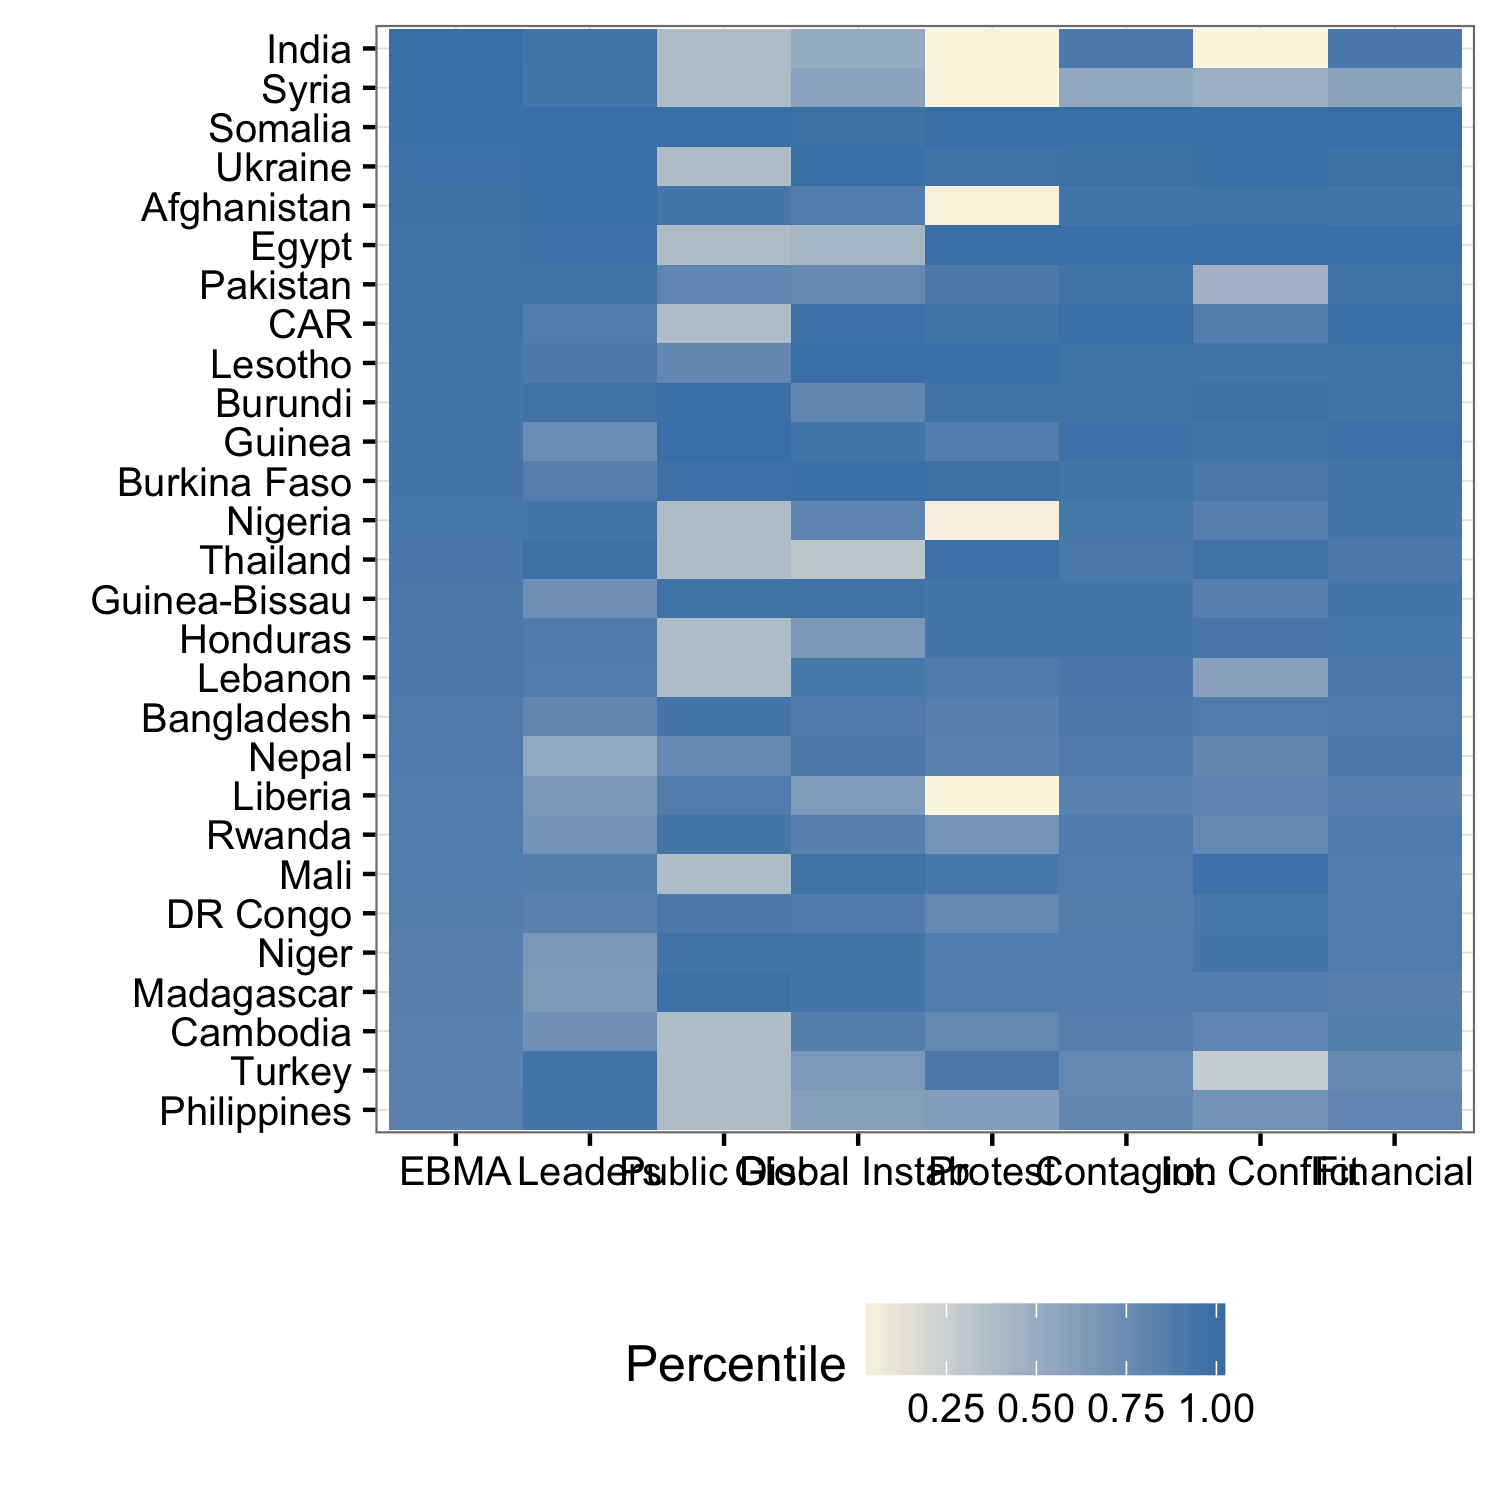
\includegraphics[width=.7\textwidth]{fcast-table}
\end{figure*}

Figure \ref{fig:predcor} visualizes the predictions for the risk of ILC in the first half of 2015 for all 165 countries for which we have complete data, for both the ensemble and 7 thematic models. The cases are ranked from highest to lowest by the ensemble prediction. Each cell represents the ensemble or theme model forecast for that country and is shaded by the probability value.\footnote{Due to the extreme differences in probability distributions between the models, it is challenging to find a single color scheme that will meaningfully represent all cases.} By comparing the cells in a row, one can get a general understanding of which model is driving an ensemble prediction, and the rank order conveys how high the risk of ILC is.

\subsection{Modeling for ensembles}

Creating models that usefully contribute to ensembles can be counterintuitive. Rather than aiming for high overall fit, the ensemble also rewards models whose predictions fill existing gaps left by other models. To identify the extent to which the predictions from the 7 models are correlated or unique, we considered two kinds figures. 

\begin{figure}
  \centering
  \caption{Calibration prediction correlations}
  \label{fig:predcor}
  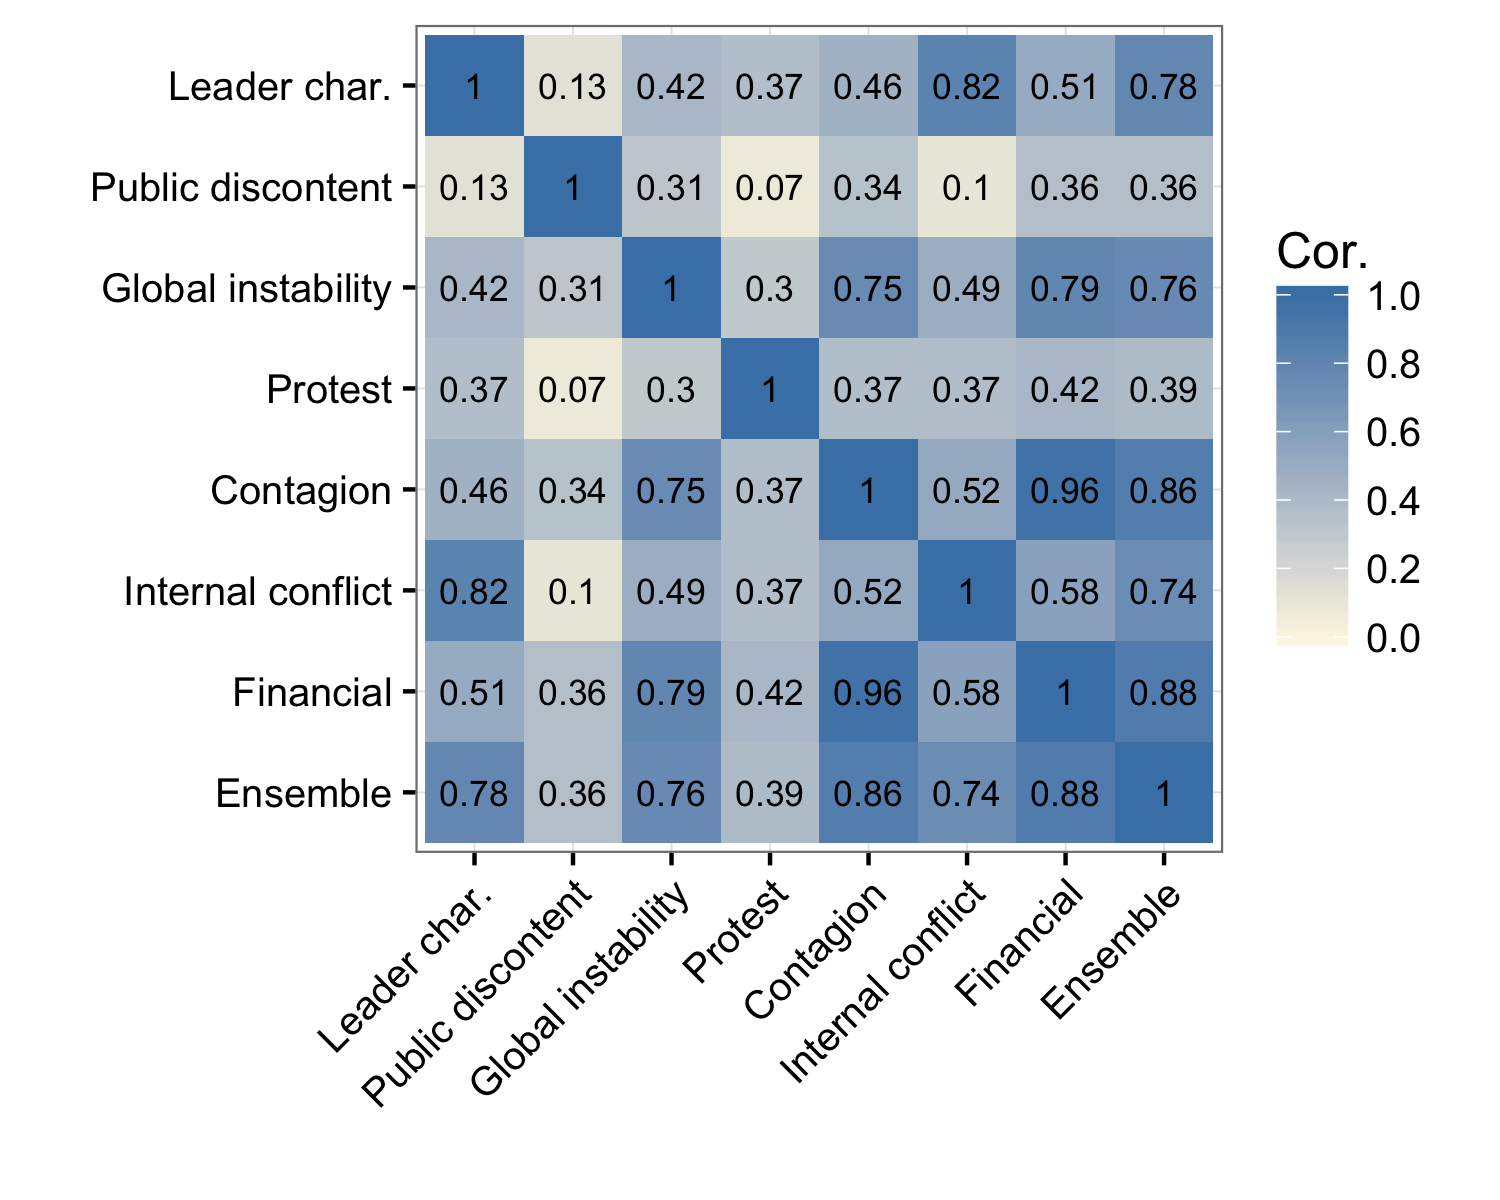
\includegraphics[width=.99\textwidth]{pred-cor}
\end{figure}

The first is a correlation plot, shown in Figure \ref{fig:predcor}. This is useful for pairwise comparisons, and shows that some theme model predictions are quite uncorrelated, but still does not help with the identification of larger gaps when considering all models together. To evaluate this we try to use plots like those shown in Figure \ref{fig:uniplot}. Similar to the forecast heat map above, these show visualize the predictions for all country-months in the data, except that the plots are now stratified by observed outcomes.

\begin{figure*}
\begin{subfigure}{.8\textwidth}
  \centering
  \caption{Calibration predictions}
  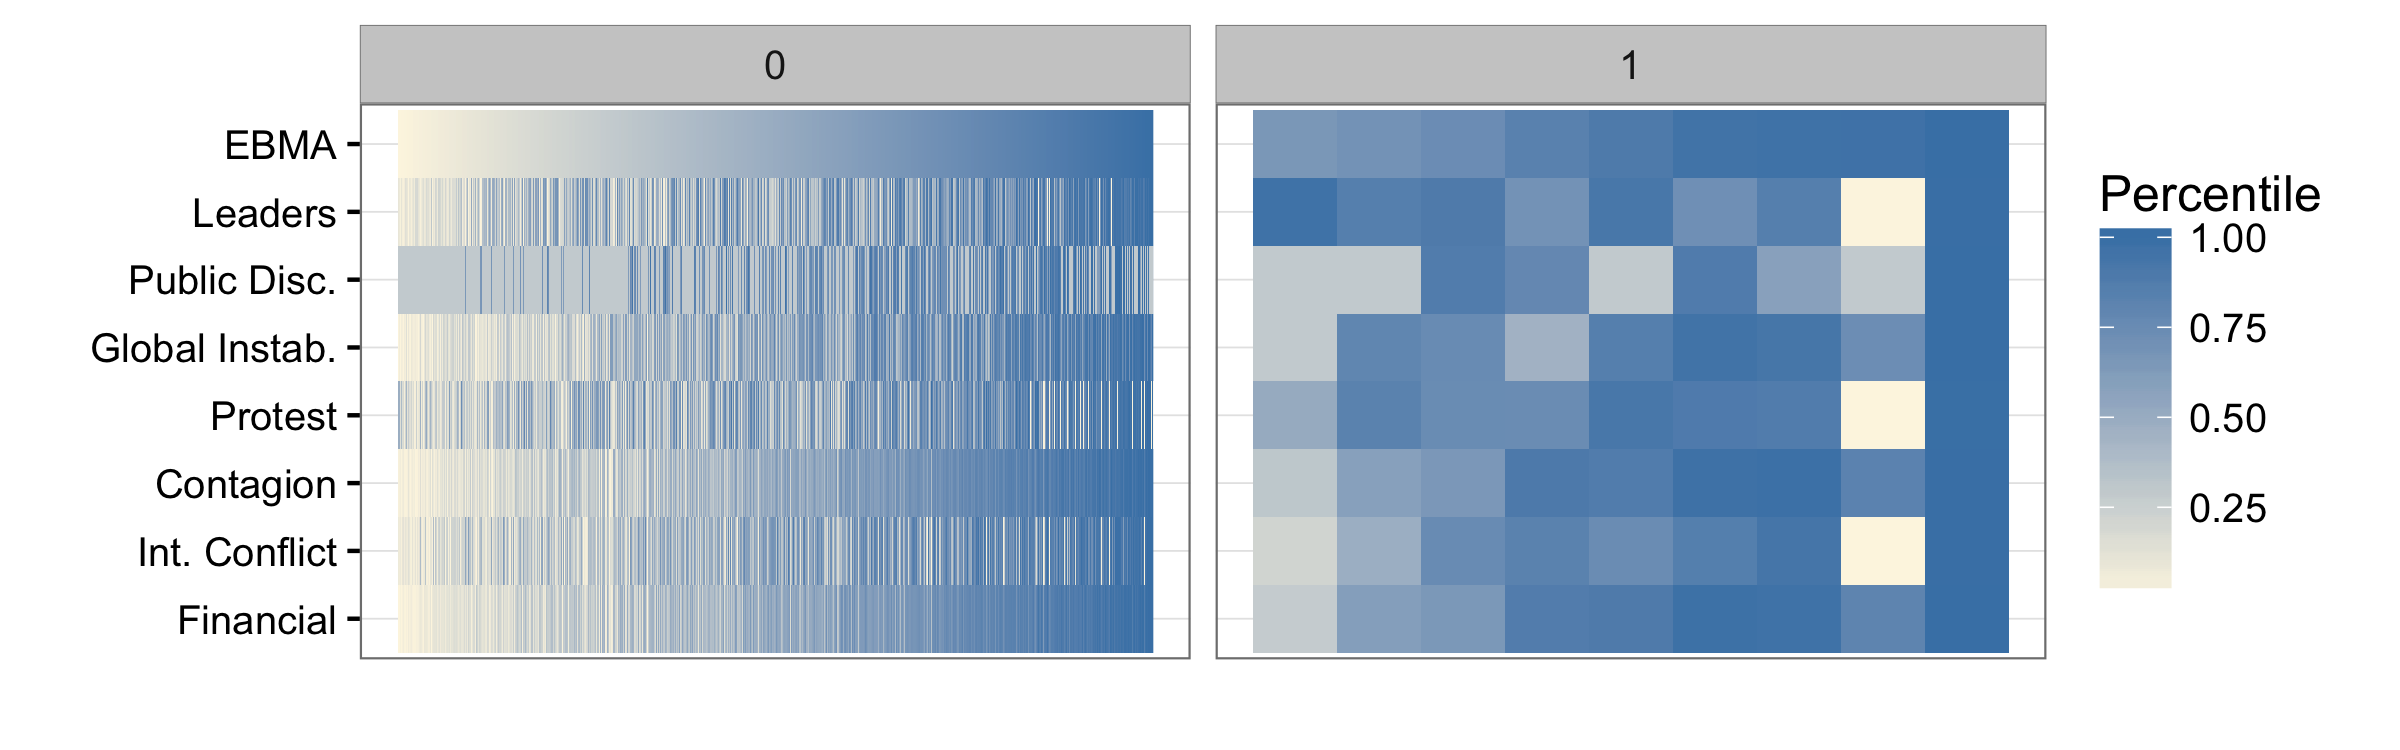
\includegraphics[width=.99\textwidth]{ebma-uniplot-calib}
\end{subfigure}
\begin{subfigure}{.8\textwidth}
  \centering
  \caption{Test predictions}
  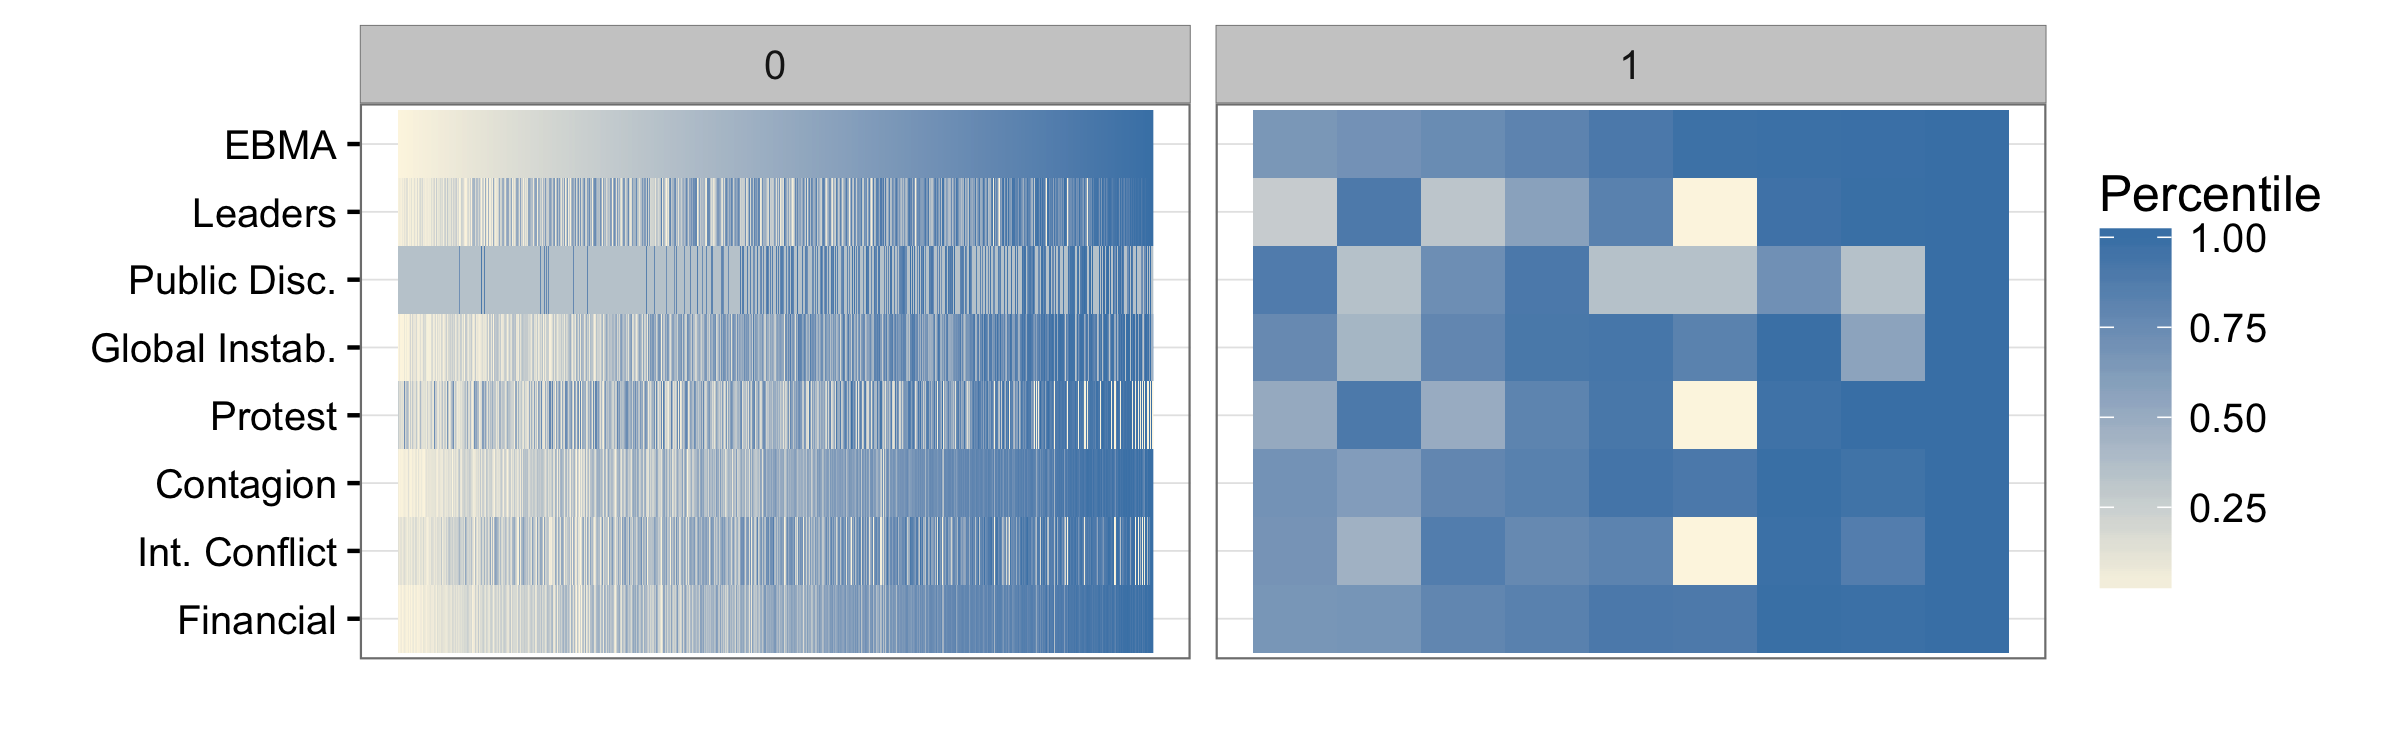
\includegraphics[width=.99\textwidth]{ebma-uniplot-test}
\end{subfigure}
\begin{subfigure}{.8\textwidth}
  \centering
  \caption{Rolling test predictions}
  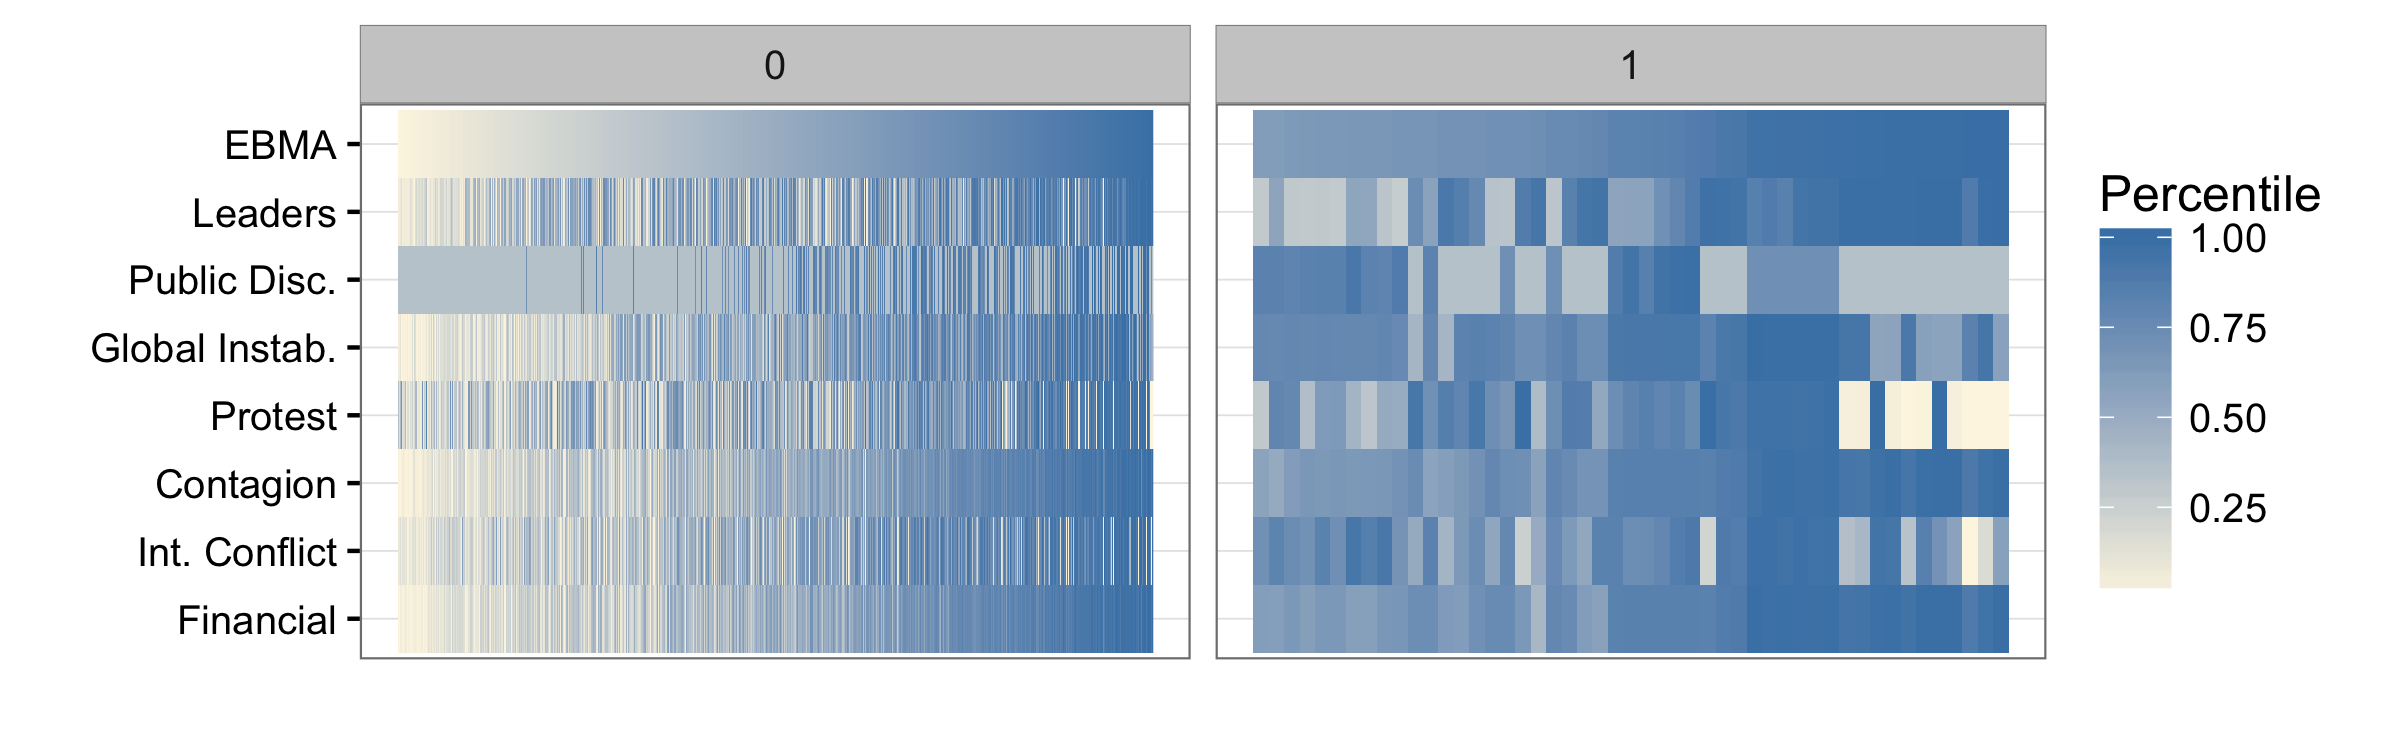
\includegraphics[width=.99\textwidth]{ebma-uniplot-test6}
\end{subfigure}
\caption{Comparison of model predictions for negative and positive outcomes.}
\label{fig:uniplot}
\end{figure*}

These plots show the variation in the extent to which the thematic predictions overlap, and we plan to use them in the future to identify gaps for further exploration and modeling. 

\subsection{Case discussions}

Lastly, several of the plots we have introduced lead to the question of which cases are examples of success for our forecasting model, and which cases are failures, either because of predictions that are too low for positive outcomes or too high for negatives. The latter are potentially very useful for identifying  shortcomings in the current suite of models. A first look at this is shown in Figure \ref{top-rank}\footnote{Note: We hope to use this plot and a similar one for Yemen in the future to further explore how our forecasts reflected the risk for these countries in light of their outcomes, and plan to also look at cases we missed, like Yemen seems likely to have been, once Archigos data are updated. }. The plot shows how highly a country was ranked for each 6-month forecast from month $t$ on the $x$-axis on. Red squares mark country-months where an ILC actually occurred, and black circles forecasts which included these ILCs in their 6-month timeframe. The countries that had an ILC over the test period are highlighted. 

\begin{figure*}
  \centering
  \caption{Forecast rank evolution over rolling 6-month test forecasts. Red squares mark country-months when ILCs occurred, black circles mark forecasts which included these ILCs.}
  \label{top-rank}
  \includegraphics[width=.99\textwidth]{top-rank}
\end{figure*}

\section{Conclusion}

Accurately forecasting ILCs at the monthly level is a difficult task, in no small part due to the sparsity of data, but also because there is much work left to do in exploring the sub-annual and higher resolution processes that drive coups, revolutions, rebellions, and other processes related to ILCs. Through continuous refinement we have been able to maintain forecasts which achieve AUC-ROC values of 0.875 and AUC-PR values of $>$0.1 while at the same time improving the out-of-sample test procedure to rolling 6-month forecasts that make us more confident that these accuracy levels truly reflect our forecasts. 

A few concluding thoughts:
\begin{enumerate}
\item A single model is unlikely to be able to capture all mechanisms and early warning indicators needed to accurately predict future events, and instead ensembles of several distinct models.
\item Creating credible forecasts that have both high recall and precision with sparse data requires AUC-ROC values that far exceed conventional expectations for good performance. Furthermore, as recall can arbitrarily be increased by loosening the threshold for making forecasts, sparse data place practical limits on precision and this is thus a avenue to pursue in future modeling. 
\item Model selection and development when the goal is to develop contributors to an ensemble while preserving transparency (unlike black-box ensembles of weak learners) is unexplored but potentially fruitful for improving forecasts. 
\item Fairly accurate forecasts, in near-real time, are possible in conflict research, as we have shown with our effort to forecast ILCs. While much work remains to be done in this domain to improve forecast precision and automation, it seems plausible to create open-source and public systems for forecasting a variety of outcomes. 
\end{enumerate}

Despite the challenges, forecasting in the end is a satisfying research task: in the end one knows whether one was wrong or right. And having this kind of feedback is rare when working with observational data, like most conflict researchers do.

\section{Replication data}

The R code used to estimate models and create the forecasts, the underlying data, and an online appendix can be found at http://www.prio.no/jpr/datasets or on github at https://github.com/andybega/jpr-ilc2015.


\clearpage

%
% 	References
%
%%%%%%%%%%%%%%%%%%%%%%%%
\bibliographystyle{apsr}
\bibliography{/Users/andybega/Work/whistle/master}
%\bibliography{/Users/mw160/git/whistle/master}

%
% 	Appendix
%
%%%%%%%%%%%%%%%%%%%%%%%%
\clearpage
\numberwithin{table}{section}
\appendix

\section{Theme model estimates}

Tables \ref{model1} through \ref{model7} show estimates for the 7 thematic models.

% latex table generated in R 3.1.2 by xtable 1.7-4 package
% Thu Apr 16 11:57:53 2015
\begin{table*}[ht]
\centering
\begin{tabular}{lrrr}
  \hline
Parameter & beta & SE & p \\ 
  \hline
(Dur. Intercept) & -1.26 & 1.69 & 0.46 \\ 
  log10(i\_matl\_conf\_DIStGOV\_l1 + 1) & -2.20 & 0.49 & 0.00 \\ 
  log10(i\_matl\_coop\_GOVtGOV\_l1 + 1) & 0.66 & 0.89 & 0.46 \\ 
  ldr\_age & 0.01 & 0.02 & 0.53 \\ 
  log10(events\_by\_mth) & 1.68 & 0.36 & 0.00 \\ 
  log(alpha) & 0.40 & 0.11 & 0.00 \\ 
  (Risk Intercept) & -15.21 & 8.88 & 0.09 \\ 
  ldr\_irregular & 13.38 & 1310.15 & 0.99 \\ 
  ldr\_foreign & -16.65 & 49.27 & 0.74 \\ 
  log10(mths\_in\_power + 1) & 0.77 & 0.94 & 0.41 \\ 
  log10(events\_by\_mth).1 & 4.65 & 2.55 & 0.07 \\ 
   \hline
\end{tabular}
\caption{Leaders} 
\label{model1}
\end{table*}
% latex table generated in R 3.1.2 by xtable 1.7-4 package
% Thu Apr 16 11:57:53 2015
\begin{table*}[ht]
\centering
\begin{tabular}{lrrr}
  \hline
Parameter & beta & SE & p \\ 
  \hline
(Dur. Intercept) & 2.26 & 1.45 & 0.12 \\ 
  log10(i\_verb\_coop\_GOVtGOV\_l1 + 1) & 1.38 & 0.51 & 0.01 \\ 
  log10(i\_verb\_conf\_GOVtDIS\_l1 + 1) & -1.61 & 0.95 & 0.09 \\ 
  log10(i\_verb\_conf\_DIStGOV\_l1 + 1) & -1.66 & 0.93 & 0.07 \\ 
  log10(i\_protest\_tGOV\_l1 + 1) & -1.19 & 0.61 & 0.05 \\ 
  log10(events\_by\_mth) & 0.88 & 0.39 & 0.02 \\ 
  log(alpha) & 0.42 & 0.10 & 0.00 \\ 
  (Risk Intercept) & 570.09 & 1608.88 & 0.72 \\ 
  IT.NET.USER.P2.l1 & -268.16 & 780.55 & 0.73 \\ 
  IT.CEL.SETS.P2.l1 & 291.40 & 852.59 & 0.73 \\ 
  log10(exclpop.l1 + 1) & 164.49 & 662.61 & 0.80 \\ 
  AUTOC.l1 & -63.55 & 178.56 & 0.72 \\ 
   \hline
\end{tabular}
\caption{Public Discontent} 
\label{model2}
\end{table*}
% latex table generated in R 3.1.2 by xtable 1.7-4 package
% Thu Apr 16 11:57:53 2015
\begin{table*}[ht]
\centering
\begin{tabular}{lrrr}
  \hline
Parameter & beta & SE & p \\ 
  \hline
(Dur. Intercept) & 2.14 & 1.13 & 0.06 \\ 
  W.knn4.std.eth.rel.h.count.l1 & 0.05 & 0.18 & 0.78 \\ 
  W.knn4.std.cw.h.count.both.l1 & -0.01 & 0.03 & 0.83 \\ 
  log10(events\_by\_mth) & 0.75 & 0.27 & 0.01 \\ 
  log(alpha) & 0.32 & 0.11 & 0.01 \\ 
  (Risk Intercept) & -3.22 & 2.17 & 0.14 \\ 
  gold\_regime\_l1FullDem & 2.20 & 1.95 & 0.26 \\ 
  gold\_regime\_l1Other & 1.51 & 1.71 & 0.38 \\ 
  gold\_regime\_l1PartAut & 20.15 & 0.00 & 0.00 \\ 
  gold\_regime\_l1PartDem & 2.08 & 1.47 & 0.16 \\ 
  gold\_regime\_l1PartDemFact & 6.77 & 3.15 & 0.03 \\ 
  log10(exclpop.l1 + 1) & 24.97 & 34.79 & 0.47 \\ 
  SH.DYN.MORT.l1norml10 & 5.99 & 2.81 & 0.03 \\ 
   \hline
\end{tabular}
\caption{Global Instability} 
\label{model3}
\end{table*}
% latex table generated in R 3.1.2 by xtable 1.7-4 package
% Thu Apr 16 11:57:53 2015
\begin{table*}[ht]
\centering
\begin{tabular}{lrrr}
  \hline
Parameter & beta & SE & p \\ 
  \hline
(Dur. Intercept) & 6.12 & 0.94 & 0.00 \\ 
  eth.rel.l.count.l1 & 4.35 & 29.00 & 0.88 \\ 
  reb.l.count.both.l1 & -0.18 & 0.05 & 0.00 \\ 
  protest.tALL.l1 & -0.01 & 0.00 & 0.09 \\ 
  W.gower.pol.reb.l.count.both.l1 & -0.03 & 0.05 & 0.60 \\ 
  log(alpha) & 0.10 & 0.22 & 0.64 \\ 
  (Risk Intercept) & -0.01 & 42.73 & 1.00 \\ 
  dom.cris.i.count.l1 & 0.14 & 0.09 & 0.10 \\ 
  log10(MS.MIL.XPND.GD.ZS.l1) & -0.22 & 1.78 & 0.90 \\ 
  log10(events\_by\_mth) & 0.03 & 8.49 & 1.00 \\ 
   \hline
\end{tabular}
\caption{Protest} 
\label{model4}
\end{table*}
% latex table generated in R 3.1.2 by xtable 1.7-4 package
% Thu Apr 16 11:57:53 2015
\begin{table*}[ht]
\centering
\begin{tabular}{lrrr}
  \hline
Parameter & beta & SE & p \\ 
  \hline
(Dur. Intercept) & 3.10 & 3.65 & 0.40 \\ 
  log10(W.centdist.std.opp\_resistance.l1 + 1) & 0.19 & 3.70 & 0.96 \\ 
  log10(W.centdist.std.repression.l1 + 1) & -0.64 & 3.35 & 0.85 \\ 
  log10(events\_by\_mth) & 0.51 & 1.10 & 0.64 \\ 
  log(alpha) & 0.27 & 0.12 & 0.02 \\ 
  (Risk Intercept) & 7.16 & 2.81 & 0.01 \\ 
  log10(SP.POP.TOTL.l1) & 2.60 & 1.31 & 0.05 \\ 
  log10(NY.GDP.MKTP.KD.l1) & -3.01 & 0.99 & 0.00 \\ 
  log10(opp\_resistance.l1 + 1) & 2.69 & 0.99 & 0.01 \\ 
  log10(events\_by\_mth).1 & -1.49 & 0.61 & 0.01 \\ 
   \hline
\end{tabular}
\caption{Contagion} 
\label{model5}
\end{table*}
% latex table generated in R 3.1.2 by xtable 1.7-4 package
% Thu Apr 16 11:57:53 2015
\begin{table*}[ht]
\centering
\begin{tabular}{lrrr}
  \hline
Parameter & beta & SE & p \\ 
  \hline
(Dur. Intercept) & 0.12 & 1.57 & 0.94 \\ 
  log(intratension.l1 * i\_protest\_tGOV\_l1 * IT.CEL.SETS.P2.l1 + 1) & 0.28 & 0.10 & 0.00 \\ 
  log(intratension.l1 + 1) & -0.57 & 0.21 & 0.01 \\ 
  log(i\_protest\_tGOV\_l1 + 1) & -0.95 & 0.18 & 0.00 \\ 
  log(IT.CEL.SETS.P2.l1 + 1) & -0.11 & 0.23 & 0.63 \\ 
  log10(events\_by\_mth) & 1.44 & 0.42 & 0.00 \\ 
  log(alpha) & 0.25 & 0.11 & 0.02 \\ 
  (Risk Intercept) & 14.34 & 3.98 & 0.00 \\ 
  log10(NY.GDP.PCAP.KD.l1) & -3.88 & 1.11 & 0.00 \\ 
  AUTOC.l1 & 0.01 & 0.03 & 0.76 \\ 
   \hline
\end{tabular}
\caption{Int. Conflict} 
\label{model6}
\end{table*}
% latex table generated in R 3.1.2 by xtable 1.7-4 package
% Thu Apr 16 11:57:53 2015
\begin{table*}[ht]
\centering
\begin{tabular}{lrrr}
  \hline
Parameter & beta & SE & p \\ 
  \hline
(Dur. Intercept) & 4.49 & 0.91 & 0.00 \\ 
  FP.CPI.TOTL.ZG.l1 $>$ 5TRUE & 0.11 & 0.46 & 0.81 \\ 
  food\_price\_idx\_l1 & 0.00 & 0.01 & 0.52 \\ 
  eu\_brent\_oil\_d1\_l1 & 0.54 & 1.98 & 0.79 \\ 
  log(alpha) & 0.28 & 0.12 & 0.02 \\ 
  (Risk Intercept) & 8.16 & 2.96 & 0.01 \\ 
  log10(NY.GDP.MKTP.KD.l1) & -2.79 & 0.83 & 0.00 \\ 
  log10(SP.POP.TOTL.l1) & 2.29 & 1.09 & 0.03 \\ 
  log10(opp\_resistance.l1 + 1) & 2.52 & 0.83 & 0.00 \\ 
  log10(events\_by\_mth) & -1.71 & 0.62 & 0.01 \\ 
   \hline
\end{tabular}
\caption{Financial} 
\label{model7}
\end{table*}


\section{List of ILCs from 1991}

Table \ref{tab:ilcs} lists all ILCs from 1991 on. It includes indicators for whether and ILC occurred due to the irregular exit or entry of a leader, or both. Due to coding convention, we list the leader who was in power when the ILC occurred, i.e. the first leader in a transition, even if the transition of irregular because an irregular entry without prior irregular exit occurred.

% latex table generated in R 3.1.2 by xtable 1.7-4 package
% Fri Mar 13 16:25:25 2015
\begin{table*}[ht]
\centering \small
\caption{List of Irregular leadership changes from 1991 to 2014}
\label{tab:ilcs}
\begin{tabular}{rlllrrl}
 \toprule
 & Country & Date & Leader & Irr. Exit & Irr. Entry & Yrs. in power \\ 
  \midrule
1 & Somalia & 1991-01 & Siad Barre & 1 & 0 & 21 \\ 
  2 & Thailand & 1991-02 & Choonhavan & 1 & 0 & 2 \\ 
  3 & Mali & 1991-03 & Traore & 1 & 1 & 22 \\ 
  4 & Ethiopia & 1991-05 & Mengistu Marriam & 1 & 1 & 14 \\ 
  5 & Lesotho & 1991-05 & Lekhanya & 1 & 1 & 5 \\ 
  6 & Russia (Soviet Union) & 1991-08 & Gorbachev & 1 & 0 & 6 \\ 
  7 & Haiti & 1991-09 & Aristide & 1 & 1 & 1 \\ 
  8 & Algeria & 1992-01 & Benjedid & 1 & 1 & 13 \\ 
  9 & Georgia & 1992-01 & Gamsakhurdia & 1 & 1 & 1 \\ 
  10 & Afghanistan & 1992-04 & Najibullah & 1 & 1 & 6 \\ 
  11 & Sierra Leone & 1992-04 & Momoh & 1 & 1 & 6 \\ 
  12 & Azerbaijan & 1992-05 & Mamedov & 0 & 1 & $<$1 \\ 
  13 & Algeria & 1992-06 & Boudiaf & 1 & 0 & $<$1 \\ 
  14 & Azerbaijan & 1992-06 & Gambarov & 0 & 1 & $<$1 \\ 
  15 & Tajikistan & 1992-09 & Nabiyev & 1 & 0 & 1 \\ 
  16 & Tajikistan & 1992-11 & Iskandrov & 0 & 1 & $<$1 \\ 
  17 & Pakistan & 1993-04 & Sharif & 1 & 1 & 2 \\ 
  18 & Guatemala & 1993-05 & Serrano Elias & 1 & 0 & 2 \\ 
  19 & Sri Lanka (Ceylon) & 1993-05 & Premadasa & 1 & 0 & 4 \\ 
  20 & Azerbaijan & 1993-06 & Abulfaz Elchibey & 1 & 0 & 1 \\ 
  21 & Guatemala & 1993-06 & Espina Salguero & 0 & 1 & $<$1 \\ 
  22 & Nigeria & 1993-08 & Babangida & 0 & 1 & 8 \\ 
  23 & Burundi & 1993-10 & Ndadaye & 1 & 1 & $<$1 \\ 
  24 & Nigeria & 1993-11 & Shonekan & 1 & 1 & $<$1 \\ 
  25 & Burundi & 1994-04 & Ntarymira & 1 & 0 & $<$1 \\ 
  26 & Rwanda & 1994-04 & Habyarimana & 1 & 1 & 21 \\ 
  27 & Gambia & 1994-07 & Jawara & 1 & 1 & 29 \\ 
  28 & Lesotho & 1994-08 & Mokhehle & 1 & 1 & 1 \\ 
  29 & Lesotho & 1994-09 & Letsie III & 0 & 1 & $<$1 \\ 
  30 & Solomon Islands & 1994-10 & Hilly & 1 & 1 & 1 \\ 
  31 & Qatar & 1995-06 & Khalifah Ath-Thani & 1 & 1 & 23 \\ 
  32 & Comoros & 1995-09 & Djohar & 1 & 1 & 6 \\ 
  33 & Israel & 1995-11 & Rabin & 1 & 0 & 3 \\ 
  34 & Niger & 1996-01 & Ousmane & 1 & 1 & 3 \\ 
  35 & Sierra Leone & 1996-01 & Strasser & 1 & 1 & 4 \\ 
  36 & Burundi & 1996-07 & Ntibantunganya & 1 & 1 & 2 \\ 
  37 & Afghanistan & 1996-09 & Burhanuddin Rabbani & 1 & 1 & 4 \\ 
  38 & Pakistan & 1996-11 & Bhutto Benazir & 1 & 1 & 3 \\ 
  39 & Congo, Dem. Rep. & 1997-05 & Mobutu & 1 & 1 & 32 \\ 
  40 & Sierra Leone & 1997-05 & Kabbah & 1 & 1 & 1 \\ 
  41 & Turkey (Ottoman Empire) & 1997-06 & Erbakan & 1 & 1 & 1 \\ 
  42 & Cambodia (Kampuchea) & 1997-07 & Ranariddh & 1 & 1 & 4 \\ 
  43 & Congo & 1997-10 & Lissouba & 1 & 1 & 5 \\ 
  44 & Comoros & 1999-04 & Massounde & 1 & 1 & $<$1 \\ 
  45 & Niger & 1999-04 & Mainassara & 1 & 1 & 3 \\ 
  46 & Guinea-Bissau & 1999-05 & Vieira & 1 & 1 & 18 \\ 
  47 & Pakistan & 1999-10 & Sharif & 1 & 1 & 3 \\ 
  48 & Cote D'Ivoire & 1999-12 & Konan Bedie & 1 & 1 & 6 \\ 
  \midrule
  \multicolumn{7}{l}{\textit{continued on next page}} 
\end{tabular}
\end{table*}
\begin{table*}
\centering \small
\begin{tabular}{rlllrrl}
\multicolumn{7}{l}{\textit{continued from previous page, 2000--2014}} \\
\midrule
 & Country & Date & Leader & Irr. Exit & Irr. Entry & Yrs. in power \\ 
  \midrule
  49 & Ecuador & 2000-01 & Mahuad & 1 & 1 & 1 \\ 
  50 & Fiji & 2000-05 & Chaudhry & 1 & 1 & 1 \\ 
  51 & Solomon Islands & 2000-06 & Ulufa'alu & 1 & 0 & 3 \\ 
  52 & Fiji & 2000-07 & Bainimarama & 1 & 0 & $<$1 \\ 
  53 & Cote D'Ivoire & 2000-10 & Guei & 1 & 1 & 1 \\ 
  54 & Congo, Dem. Rep. & 2001-01 & Laurent Kabila & 1 & 0 & 4 \\ 
  55 & Afghanistan & 2001-11 & Mullah Omar & 1 & 0 & 5 \\ 
  56 & Madagascar & 2002-07 & Ratsiraka & 1 & 1 & 5 \\ 
  57 & Central African Republic & 2003-03 & Patasse & 1 & 0 & 9 \\ 
  58 & Guinea-Bissau & 2003-09 & Kumba Iala & 1 & 1 & 4 \\ 
  59 & Georgia & 2003-11 & Shevardnadze & 1 & 0 & 12 \\ 
  60 & Haiti & 2004-02 & Aristide & 1 & 0 & 3 \\ 
  61 & Kyrgyz Republic & 2005-04 & Akayev & 1 & 0 & 14 \\ 
  62 & Bolivia & 2005-06 & Carlos Mesa & 1 & 0 & 2 \\ 
  63 & Mauritania & 2005-08 & Sidi Ahmed Taya & 1 & 1 & 21 \\ 
  64 & Nepal & 2006-04 & Gyanendra & 1 & 0 & 1 \\ 
  65 & Solomon Islands & 2006-05 & Rini & 1 & 0 & $<$1 \\ 
  66 & Thailand & 2006-09 & Thaksin Shinawatra & 1 & 0 & 6 \\ 
  67 & Fiji & 2006-12 & Laisenia Qarase & 1 & 0 & 6 \\ 
  68 & Bangladesh & 2007-01 & Iajuddin & 1 & 0 & $<$1 \\ 
  69 & Fiji & 2007-01 & Senilagakali & 0 & 1 & $<$1 \\ 
  70 & Georgia & 2007-11 & Saakashvili & 1 & 0 & 4 \\ 
  71 & Lebanon & 2008-05 & Siniora & 1 & 0 & $<$1 \\ 
  72 & Mauritania & 2008-08 & Ould Cheikh Abdellahi & 1 & 1 & 1 \\ 
  73 & Guinea & 2008-12 & Conte & 0 & 1 & 25 \\ 
  74 & Guinea-Bissau & 2009-03 & Vieira & 1 & 0 & 3 \\ 
  75 & Madagascar & 2009-03 & Marc Ravalomanana & 1 & 1 & 7 \\ 
  76 & Honduras & 2009-06 & Zelaya & 1 & 1 & 3 \\ 
  77 & Guinea & 2009-12 & Dadis Camara & 1 & 1 & 1 \\ 
  78 & Niger & 2010-02 & Mamadou & 1 & 1 & 10 \\ 
  79 & Kyrgyz Republic & 2010-04 & Bakiyev & 1 & 0 & 5 \\ 
  80 & Tunisia & 2011-01 & Zine Al-Abidine Ben Ali & 1 & 0 & 23 \\ 
  81 & Egypt & 2011-02 & Mubarak & 1 & 0 & 29 \\ 
  82 & Cote D?Ivoire & 2011-04 & Laurent Gbagbo & 1 & 1 & 10 \\ 
  83 & Libya & 2011-08 & Qaddafi & 1 & 1 & 42 \\ 
  84 & Mali & 2012-03 & Amadou Toure & 1 & 1 & 10 \\ 
  85 & Guinea-Bissau & 2012-04 & Raimundo Pereira & 1 & 1 & $<$1 \\ 
  86 & Mali & 2012-04 & Amadou Sanogo & 0 & 1 & $<$1 \\ 
  87 & Central African Republic & 2013-03 & Francois Bozize & 1 & 1 & 10 \\ 
  88 & Egypt & 2013-07 & Morsi & 1 & 1 & 1 \\ 
  89 & Central African Republic & 2014-01 & Djotodia & 1 & 0 & 1 \\ 
  90 & Ukraine & 2014-02 & Yanukovych & 1 & 0 & 4 \\ 
  91 & Thailand & 2014-05 & Yingluck Shinawatra & 0 & 1 & 3 \\ 
  92 & Burkina Faso (Upper Volta) & 2014-10 & Campaore & 1 & 1 & 27 \\ 
  93 & Burkina Faso (Upper Volta) & 2014-11 & Traore & 1 & 1 & $<$1 \\ 
   \bottomrule
\end{tabular}
\end{table*}

%
%	Bio sketches:
%
%The biosketch in JPR appears immediately after the references. It should be brief and include year of birth, highest academic degree, year achieved, where obtained, position and current institutional affiliation. In addition authors may indicate their present main research interest or recent (co-)authored or edited books as well as other institutional affiliations which have occupied a major portion of their professional lives. But we are not asking for a complete CV.
%Sample biographies:
%IVER IVERSEN, b. 1976, Cand. Polit. (University of Oslo, 2002); Secretary, Norwegian Ministry of Foreign Affairs (2002?04); University Fellow in Political Science, University of Oslo (2004? ); current main interest: global political economy. Most recent book in English: Globalization and Conflict (Sage, 2005).
%ABDULAH NASSA, b. 1947, PhD in Economics (University of Michigan, 1966); Associate Professor, Florida State University (1964? ); various visiting academic positions in Sudan, India, and Britain. Most recent book: Economics of Crime (Harper & Row, 1996).
%Note the use of capital initials for subjects (Economics, Political Science), degrees (Cand.Polit.), and positions (Assistant Professor). No full stops in PhD, MA, MSc, etc.
%
%%%%%%%%%%%%%%%%%%%%%%%%%

ANDREAS BEGER, b. 1983, PhD in Political Science (Florida State University, 2012); Independent Consultant (2015--); Postdoctoral Associate, Duke University (2012-2015).

MICHAEL D. WARD


%
%	Document end
%
%%%%%%%%%%%%%%%%%%%%%%%%%
\end{document}